\documentclass{report}
\usepackage[
backend=biber,
style=nature,
]{biblatex}
\addbibresource{references.bib} %Import the bibliography file
\usepackage{graphicx} % Required for inserting images
\usepackage{float}
\usepackage{booktabs}
\usepackage{longtable}
\usepackage{tablefootnote}
\usepackage{pdfpages}
\usepackage{caption}
\captionsetup[figure]{font=footnotesize}

%\title{Accelerating sporting expertise through effectice learning problems and teaching signals}
%\title{Making the hours count: can we improve skill learning by using more effective learning problems and more effective teaching signals?}
%\title{Skill learning in elite athletes: can we improve skill learning by using more effective learning problems and more effective teaching signals?}
\title{Bridging laboratory and real-world skill learning: Can we teaching strategies to improve skill learning in skilled athletes}


\author{Christian Magelssen}
\date{January 2024}

\begin{document}
\newcommand{\RNum}[1]{\uppercase\expandafter{\romannumeral #1\relax}}


\maketitle

\tableofcontents 
\listoffigures


\chapter{Introduction}

Doktorgradsprosjektet er et samarbeidsprosjekt mellom the Norwegian School of Sport Sciences (Department of Physical Performance), the Norwegian Ski Federation, SNØ (the indoor ski hall in Oslo) og skigymnas og klubber i Norge og Sverige. Jeg er takknemlig for muligheten dere har gitt meg til å gjøre et slikt prosjekt som dette, og jeg håper jeg har klart å levere tilbake til dere med praktisk anvennelig kunnskap, men som også er av teoretisk interesse for psykologifaget. 

Det er en rekke mennesker som skal har hjulpet med på veien og som fortjener en stor takk.

Romy Frömer: Jeg er veldig glad for at jeg spurte deg om hvordan du hadde laget dine figurer til din elife artikkel, og at du spurte meg "er det noe mer jeg kan hjelpe deg med?" etter at du hadde forklart meg hvordan du laget slike figurer. Det gjorde at jeg muligheten til å presentere noen tanker rundt reinforcement learning i alpint. Siden dette har vi jobbet sammen, og du ble formelt min veileder høsten 2023. Jeg umåtelig takknemlig for måten du har veiledet meg på gjennom ukentlig mandagsmøter og tett oppfølging. Du har trent meg i vitenskapelig tenkning, open science og skriving.  

Per Haugen: Takk for all hjelp du har gjort med doktorgraden. Du har vært en enestående sparringspartner gjennom alle mine år på NIH-fra bacelor til doktorgradsstudiet. Din dør har alltid står åpen, og har vært en person jeg alltid kan ringe om jeg står fast, enten det er med å forskning eller at jeg sliter med en polish som ikke vil heve. Du er den mest kunnskapsrike personen om alpint. 

Robert Reid: Takk for sparringen vi har hatt rundt prosjektene-fra bachelor til doktorgrad, og at du har støttet og forankret prosjektet i Norges skifobund sin FOU strategy. 

Thomas Losnegard: Takk for at du har vært genuint interessert i motorisk læring og har støttet prosjektet gjennom hele min doktorgrad. Dine råd om å holde ting enkelt og gjennomførbart har vært avgjørende for at jeg har kommet i mål. 

Matthias Gilgien: Takk for at du formelt var min veileder. Takk for ditt bidrag under datainnsamling. 


I tillegg er det mange hjelpere som har jobbet døgnet rundt for at jeg skal få gjort prosjekene. Flere har hatt alarmen på kl 2am  for i flere uker i strekk for å få komme tidlig nok i skihallen for å rigge klart til utøverne. 

Rune Velta, Petter Husevåg Jølstad, Jasper Bates, Andreas Lodden, Kasper Sjøstrand, Kjersti Mejdell Styrmoe, Andreas Lodden, Johan Ansnes, Magne Lund-Hansen, Einar Witteveen, Allan Henriksen, Tom Knudsen, Victoria S Placth, Sara Stensø, Ørjan Lydersen, Eirik Knutsen, Haakon Staff, Live Luteberget, Sindre Lindstad Hoholm, Aurora Haug, Tor-Magnus Blakstad Cappelen, Katrine Groth Eggar, Mai Sissel Linløkkel, Simen Leithe Tajet, Erland Vedeler Stubbe, Erland Hoff Thommasen, Jeremy Phyffer, Tim Gfeller, Andreas Kollenborg, Pernille Lindemann, Tommy Akselsen, Knut Johan Bere, Tobias Torrissen, Kristrun Gudnadottir, Synne Sofie Stangeland, Brede Barkenes, Armin Triendl, Tim Gfeller, Jukka Leino, William Farstad Olsen.

Det er noen som jeg må takke mye. 



Jeg har også lyst til å takke gode kollegaer på Oslo Nye Høgskole. Først av alt vil jeg takke Randi Bjøntegaard som ville ha meg til å revidere og undervise i kognitiv psykologi sammen med Johanna Katarina Blomster Lyshol. Senere var det Andreas Berg Krosby og Pernille Krog Torp som overtok og ble min nærmeste ledere. Tusen takk for at dere begge alle har vært så støttende og tålmodige med meg. Dette gjorde at jeg hadde det helt topp hos dere. Jeg må også takke Axel Davies Vittersø og Sofie Sagfossen for at jeg fikk dele kontor med dere. Jeg er også takke Peder M Isager for alle diskusjoner om effektstørrelser og ekvivalenstesting. 

Jeg vil også takke venner og kollegaer ved Høgskolen i Innlandet (avdeling Lillehammer). Her vil jeg spesielt takke Sjur Fortun Øfsteng, Knut Sindre Mølmen, Daniel Hammarström, Heidi og Nicki Almquist for god hjelp og støtte under doktorgraden. 

Jeg må også takke Mor og Far for støtten gjennom hele livet og gjennom doktorgraden. Dere har vært noen fantastiske foreldre, som har introdusert meg for mange idretter. Uten dette hadde jeg aldri fullført doktorgraden i idrettsvitenskap. 

Jeg har 


Jeg vil også takke min Twitter/X venner for å ha hjulpet meg gjennom doktorgraden og besvart metode og statististikk spørsmål som jeg har lurt på. Jeg vil her spesielt trekke frem Isabella G. Ghement, Dale Barr, Dan Quintana, Gavin Simpson, Cameron Patrick, Solomon Kurz, James Steele, Peder M Isager, Stephen Wild, Brad McKay, Matthew Kay, Brenton Wiernik, Joseph Bulbulia og Daniël Lakens. Det tok noen år ut i doktorgraden før jeg turte å stille "dumme" spørsmål, men jeg skjønte at det er sånn de beste lærer. Jeg er glad jeg turte og stille disse "dumme" spørsmålene, og at dere var tålmodige, støttende og at dere tok dere tid til å svare. Tusen takk!

Til slutt må jeg takket min kjære samboer og forlovede Kjersti Mejdel Styrmoe. Vi ble sammen da jeg begynte på doktorgraden, på et tidspunkt der jeg var naiv nok til å tro at doktorgraden skulle bli en enkel oppgave. Du har vært min viktigste støttespiller gjennom disse 4.5 årene, og har ikke bare støttet meg på hjemmebane. Du har faktisk stilt opp på datainnsamling og stått flere dager i fryseboksen for at jeg skulle komme i mål. Jeg vet du er lei av at jeg ligger metode og statistikkbøker overalt i leiligheten, og at jeg alltid har med en ny statistikkbok på ferie hver sommer. Jeg lover at fra nå av skal disse stå i hyllene. D




\chapter{Introduction}

Humans show a remarkable ability to learn new skills, such as driving a car or skiing down an easy slope after just a few hours of practice. But beyond these everyday skills, there also exists an upper level of performance that only the fewest of us attain—such as playing in the Wimbledon tennis finals—and that is achievable only through many years of dedicated practice \cite{hodges_predicting_2004, ericsson_role_1993, vaeyens_talent_2009}. Skill learning can thus be viewed not only as a process of becoming competent but also as one that can be extended to achieve extraordinary skills \cite{ericsson_development_2003, ericsson_scientific_1998}. Understanding how some individuals make the leap from this initial competence to become experts and whether there are learning strategies that may accelerate this transition has long intrigued scientists across various disciplines \cite{ericsson_expert_1994, ericsson_scientific_1998, ericsson_development_2003, ericsson_prospects_2002} and has significant implications for many aspects of life.

In recent decades, cognitive science has made great strides in understanding the mechanisms that likely exert control of skill learning and how they can be leveraged to improve learning and performance \cite{wolpert_principles_2011, makino_circuit_2016, spampinato_multiple_2021, krakauer_motor_2019, haith_model-based_2013, huang_rethinking_2011, shmuelof_are_2011, doya_complementary_2000}. Most of these studies have leaned toward simple, laboratory-based learning tasks\cite{krakauer_motor_2019, du_relationship_2022}, such as button/ball pressing \cite{hardwick_time-dependent_2019, vassiliadis_reward_2021} or reaching movements\cite{shadmehr_adaptive_1994, krakauer_learning_2000},  which enable scientists to dissect and closely examine the contributions of individual learning mechanisms in a controlled environment \cite{spampinato_multiple_2021}. But their advantage also comes with a cost; they are unlikely to capture the full complexity of real-world skill learning \cite{krakauer_motor_2019, mangalam_investigating_2023, du_relationship_2022, chen_effects_2018, wolpert_principles_2011, gallivan_decision-making_2018, iyer_probing_2020, ingram_naturalistic_2011}. Therefore, an outstanding question is whether insights from these studies have brought us closer to understanding and improving the learning of real-world skills, which engage all learning mechanisms simultaneously \cite{spampinato_multiple_2021}. Bridging the gap between laboratory and real-world learning has thus been identified as a critical direction for future research to learn whether these theories have practical applications in natural environments, such as sports, education, and rehabilitation \cite{du_relationship_2022, wolpert_motor_2010, yarrow_inside_2009, haar_motor_2020, ingram_naturalistic_2011}.

Elite sports offer an exciting test domain for these theories because they present one of the most demanding learning challenges for the brain \cite{walsh_is_2014}. First, elite athletes must learn to optimize their performance across many situations and conditions\cite{mangalam_investigating_2023, du_relationship_2022, krakauer_motor_2019}. The need for this adaptability is one reason why achieving elite status requires many years of training \cite{krakauer_motor_2019}, in stark contrast to simpler laboratory tasks where participants reach peak performance after just minutes, hours, or days of training, and researchers already know the best solution. Second, sports involve full-body movements, unlike laboratory tasks, which typically involve only one or a few degrees of freedom \cite{du_relationship_2022}. Finally, sports are not trivial activities but generally hold intrinsic value for athletes, as they constitute an important part of their life. Therefore, athletes are generally motivated to improve their skills. Together, these characteristics make elite sports a unique and compelling domain for testing these learning theories.

Studying skill learning in elite athletes presents its own methodological challenges, however. By definition, elite athletes are already highly skilled and are expected to show minimal improvement by repeating their automated solution with additional training\cite{ericsson_development_2003, ericsson_expert_1994, ericsson_scientific_1998}. Consequently, learning experiments targeting familiar solutions are unlikely to bring improvement in performance, making elite sports an unsuitable domain for studying skill learning processes  \cite{thorndike_educational_1913, ericsson_development_2003, grayloooooong, grayshort, ericsson_scientific_1998}. However, this obstacle can be overcomed by rethinking the approach taking to the learning experiments. Often, the reason elite athletes do not progress is their lack of knowledge about better methods to solve tasks \cite{grayloooooong, grayshort, thorndike_educational_1913}. Therefore, developing strategies that help athletes improve task performance could significantly enhance their skills and is essential for testing learning theories on this skilled cohort of athletes. 
%However, this lack of improvement does not mean skilled performers cannot improve. Often, their limited performance improvement reflects a plateau caused by a lack of knowledge about better methods to solve the task. Helping athletes discover better strategies can enable them to overcome these limits and ensure performance advancement. Therefore, a necessary condition for conducting learning experiments with skilled athletes is finding ways to make them improve their skill.

Due to the necessity of finding ways to improve elite athletes' skills, this doctoral project has two overarching goals. On the one hand, it seeks to identify areas where elite athletes can improve and build knowledge and understanding of strategies they can use to achieve this. On the other hand, it aims to use this knowledge to conduct learning experiments that test cognitive science theories to enhance elite athletes' training. To synthesize these typically distinct domains of research, the project draws inspiration from the expert performance approach as a systematic framework to guide the questions for this doctoral project. This approach involves three stages. In the first stage, the focus is on identifying the areas that distinguish highly skilled from less skilled athletes. The second stage seeks to understand the mechanisms that explain these differences. Finally, the third stage examines whether these mechanisms can be explained through differences in training, which can be investigated through training history or experimental learning studies. Our approach is broader than the expert performanc approach because we aim not only to understand the mechanisms underlying elite performers' superior achievements but also to identify what athletes can do to enhance their performance and how we can improve training to achieve this. 

This doctoral project is all concentrated on alpine skiing due to the sport's high demands for skilled execution of well-chosen strategies. These strategies must be continuously adapted to changing situations, such as course settings, terrain, equipment, snow conditions, and weather. These varied situations make it nearly impossible for skiers or coaches to determine the best strategy at any given time, which makes alpine skiing a relevant test domain due to its inherent uncertainty. A secondary reason is the longstanding and close collaboration between the Norwegian School of Sport Sciences and the Norwegian Ski Federation, which has fostered mutual knowledge development about the sport.

The aim of the doctoral project was to identify key sections in a slalom course that differentiate skilled from less skilled skiers and then use this section to answer two overarching questions: What can skiers do to ski faster in this section, and how should we teach to best facilitate learning these skills? To test whether cognitive science learning theories can enhance training compared to traditional teaching strategies, the doctoral project focuses on current coaching practices and the opportunities coaches have to create constructive learning situations. 

\section{Structure of the thesis}
The structure of this doctoral thesis is closely organised around these two main questions. Following this general introduction, I will present the background for my doctoral project. In background chapter I will first argue for the specific course section I have focused my doctorate on: a section of a slalom course where significant performance differences between athletes have been observed. Next, I present strategies that could enhance the performance of skilled skiers in these sections in slalom, which may also explain these performance disparities between skiers in this section today. In the final section of that chapter, I will introduce learning theories from cognitive science that have proven effective in simple laboratory tasks, and that have the potential to improve training of athletes. Given that this doctoral research aims to test whether these theories can improve existing contemporary teaching strategies, the focus will be on how coaches can foster learning in the field and how these theories can enhance current practices. This introduction and background chapter will conclude with the research aims and questions I seek to address in this doctorate.

This doctoral research comprises two learning experiments, referred to as Study 1 and Study 2. Study 1 resulted in two papers, designated Paper 1 and Paper 2. Study 2 led to Paper 3. Additionally, data from this learning experiment were used to estimate the effects of the various strategies tested, although this analysis is not published in a paper but is presented in the results and discussion chapter of this dissertation. The results and discussion are organized around the two primary questions of the doctoral project: how can athletes improve their performance, and how should they learn these improvements? Following this discussion, I will provide a general discussion, synthesizing the studies as a whole and including a methodological discussion.

%går vi gjennom hva som skjer skiller eliteutøvere fra mindre skilled utøvere. Det neste spørsmålet er hvilke strategier som er effektive for å kjøre raskt på flater. Her går vi gjennom mekanikken for noen strategegier som kan bidra til å kjøre raskt på flater. I siste spørsmål stiller vi hva en effektive læringsparagigmer for å forbedre treningen til eliteutøvere. Til slutt forsøker vi 


%Following this general introduction, the Background presents the context of the thesis
%regarding training prescription and adaptations to resistance training. Data from two
%training interventions are presented under Methods and Results and Discussion, referred to
%a%s Study I and Study II. Results from Study I have been published as Paper I and II, and
%results from Study II are presented in Paper III. In addition to experimental results, a meta-
%analysis examining the effects of resistance training volume on muscle mass and strength
%gains is presented under Results and Discussion. Under Methodological Considerations,
%selected topics related to the experimental data used in the thesis are discussed


\chapter{Background}

\section{Where do big time differences arise between slalom skiers? }
The goal for alpine skiers is to ski a slalom course marked by gates in the shortest possible time. These slalom courses never consist of a single situation repeated from turn to turn. Instead, they include various sections with different terrains and incline angles, gate placements, snow conditions, winds, and visibility. Consequently, no two turns are the same, and the skiers must master a vast array of situations to perform well. 

At first glance, the differences between the top skiers and the next-best skiers might seem marginal. For instance, it is not uncommon for the gap between the best performer and the next ten competitors to be less than a second on a 50-second slalom course. A natural assumption is that these small differences are consistent throughout the course. However, a closer examination of specific sections of the course—through gate-to-gate analysis or shorter intermediate section analysis—reveals significant disparities in certain segments\cite{supej_relations_2006, reid_kinematic_2010, supej_new_2011, supej_mechanical_2011, federolf_quantifying_2012}. These differences suggest that athletes have both strong and weak areas that can be targeted and improved through training.

Previous slalom studies have identified three crucial sections: the start, the hairpins, and the flat sections\cite{supej_new_2011}. Among these, the flat section typically makes up the largest proportion of the total course (see Fig. \ref{fig: flatcourse} for an illustration). Consequently, improvements in this section could have a more substantial impact on a skier's overall performance compared to the start or hairpin turns. Furthermore, strategies effective on flat terrain may be applicable to hairpin turns. Therefore, for my doctoral project, I chose to focus on the flat section as the area for further study.

\begin{figure}
    \centering
    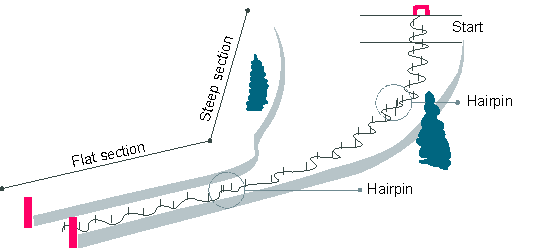
\includegraphics[width=1\linewidth]{figure/figure_introduction_course.pdf}
    \caption{Illustration of different section in a slalom race}
    \label{fig: flatcourse}
\end{figure}

\section{What can skiers do to improve their performance in flat sections in slalom?}
The next question is how skiers can increase their speed on flat sections in slalom. In this sport, performance boils down to how effectively athletes can utilize the mechanical energy available to them \cite{supej_differential_2008, supej_how_2010}. Therefore, this section first outlines the fundamental mechanical energy principles of skiing. Based on these principles and quantitative evidence from field research on elite skiers, I will propose four strategies to potentially enhance skier performance on flat terrain in slalom, which we wanted to study in this doctoal project.  

\subsection{Energy mechanics of alpine skiing}\label{introduction: energymechanics}
When skiers take the ski lift to the top, they  accumulate gravitational potential energy. This acquired potential energy is the skier's main engine \cite{supej_differential_2008, supej_mechanical_2011} and enables them to do work such as making the ski penetrate the snow to make it turn. The amount of potential energy available to the skier for performing such work at the top of a slalom course can be derived from the following equation:
\[U=mgh\]
Here, $U$ represents the gravitational potential energy (measured in joules), $m$ represents the mass of the skier (measured in kilograms), g represents the gravitational acceleration (approximately $m/s^2$) acting on the skier, and $h$ represents the height (measured in meters). When the skier descends the slalom course, the amount of work done by gravity can be derived by finding the gravitational potential energy for the initial position $U_1$ (e.g., at the top of the slalom course) and the gravitational potential energy for the final position $U_2$ (e.g., at the end of the first turn); then, the negative change in potential energy can be calculated: 
\[W=-U_2 + U_1\]
\[W= -\Delta U \]
This quantity represents the work of gravity on the skiers as they descend from the top to the lower position of the slalom course. According to the law of conservation of mechanical energy, all this work must be converted to kinetic energy when gravity is the sole force acting on the skier. The skiers' kinetic energy can be represented by the following equation:
\[ K = \frac{1}{2} m v^2 \]
where $K$ is the kinetic energy, $m$ is the mass of the skier, and $v$ is the velocity of the skier. Consequently, the sum of the potential and kinetic energy  (denoted as $E$ for mechanical energy) remains constant during a descent, as expressed by the following equation:
\[ E = U + K \]
During descents, however, skiers are exposed to two dissipative forces that oppose motion and can result in some loss of energy transfer to kinetic energy. For skiers, these two dissipative forces are air drag and snow friction (collectively denoted as $D$)\cite{supej_differential_2008}. Therefore, the total mechanical energy during a descent equals the sum of the kinetic energy and the dissipating forces (equation below), and is conceptually illustrated in Fig. \ref{fig:energy}.
\[ U = K + D\]
Consequently, in terms of the mechanical energy principle, a skier's goal during a descent should be to maintain high kinetic energy \cite{supej_differential_2008, supej_mechanical_2011, supej_how_2010}. One conventional strategy that most skilled skiers' employ to achieve this goal include carving instead of skidding \cite{supej_differential_2008, supej_relations_2006, reid_kinematic_2010, reid_turn_2009}. Are there solutions that can effectively improve performance on this section beyond the usual strategy? 

\begin{figure}[H]
    \centering
    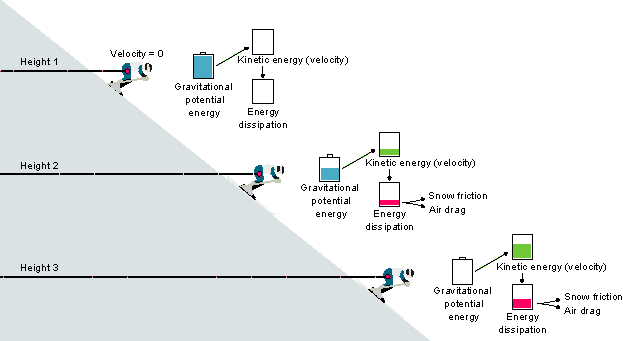
\includegraphics[width=1\linewidth]{figure/figure_introduction_mechenergy3.pdf}
    \caption{Illustration of mechanical energy in alpine skiing}
    \label{fig: energy}
\end{figure}



\subsection{Strategies to improve race times in flats in slalom}\label{introduction: strategies}
If most skilled skiers can execute clean, carved turns, what else can they do to achieve better performance on flats in slalom? Here, I outline four strategies that can potentially achieve this goal, all directed at improving energy mechanics management.  Fig. \ref{fig: strategies} illustrates these four strategies.  

The first strategy skiers could potentially use to maintain high kinetic energy during a turn and therefore improve their race times on flat sections in slalom is the 'stand against' technique. This strategien er nokså utbredt blant trenere i skimiljøet, og går ut på at skiers maintain a stable stance and actively resist being compressed toward their bindings by centrifugal force during a turn (from the skier's frame of reference). According to Lind and Sander's theoretical model on 'pumping to increase velocity' \cite{lind_physics_2004}, this active force resistance could minimize skiers' kinetic energy loss during a slalom turn by keeping the moment of inertia about the axis of rotation fixed instead of increasing it, as would occur if the skier collapsed during the turn. In their model, the rotational kinetic energy of a ski turn can be represented by the following equation: 
\[ T = \frac{L^2}{2I} \]
Here, $T$ represents the kinetic energy of rotation, and $L$ represents the angular momentum (that is, angular velocity ($\omega$) multiplied by the moment of inertia about the axis of rotation ($I = mr^2$)). Lind and Sanders considered a rider traveling on a cart on a friction-free rail with a curved turn and no torque to act on the system. In this situation, if the rider were to collapse toward the cart due to the centrifugal force, the moment of inertia would increase by lengthening the radius about the axis of rotation. Consequently, some rotational kinetic energy is lost if the skier fails to resist the centripetal force. Stand against might therefore be an effective strategy to ski faster on flats in slalom.  

A second and perhaps better strategy skiers can employ to maintain high kinetic energy during a turn is to 'rock skis forward'. By shifting their vertical position forward and backward, skiers regulate the ski’s total pressure distribution exerted against the snow\cite{lemaster_skiers_1999, lemaster_ultimate_2010, howe_new_2001}. This regulation not only helps skiers maintain balance but also affects the ski's turning behavior. For example, when skiers edge their skis, moving the center of mass toward the tip of the ski increases the pressure distribution on the ski's forebody, enabling it to turn more sharply. Conversely, if skiers edge their skis but shift their center of mass backward to the ski's tail, they decrease the pressure at the ski's forebody and consequently make the turn more gradual \cite{lemaster_skiers_1999, lemaster_ultimate_2010}. In ski racing, skiers generally aim to turn more sharply in the beginning and during the turn and should therefore shift their center of mass to distribute the pressure to the ski's forebody to make it engage with the snow. However, after gate passage, skiers generally aim to stop turning and should therefore shift their center of mass backward by rocking the skis forward. By rocking the skis forward after gate passage, skiers could in principle counteract the unnecessary loss of kinetic energy caused by the skis penetrating and digging unnecessarily into the snow in the exit of the turn. In support of this, previous research has found a strong linear relationship between the skier's forward position and energy dissipation \cite{reid_turn_2009, reid_kinematic_2010}. Additionally, faster skiers have shown to rock their skis more forward and pressure the back part of the ski for considerably longer during a turn compared to slower skiers\cite{reid_kinematic_2010, tjorhom_beskrivelse_2007}. Consequently, rocking skis forward could be an even better strategy than the stand against strategy for improving race times on flat terrain in slalom. 

The third strategy that can potentially make skiers faster on flat slopes in slalom is to 'extend,' also referred to as 'pumping' to increase velocity \cite{lind_physics_2004}. This strategy involves skiers moving their center of mass closer to the axis of rotation of a turn from a laterally inclined position by extending their legs. When the skiers extend this way, they can increase their kinetic rotational energy under certain situations. According to Lind and Sanders \cite{lind_physics_2004} model, the skier achieves this effect by shortening the radius of the axis about which they rotate, which will reduce the moment of inertia and consequently increase the rotational kinetic energy of the system under the assumption that angular momentum is conserved. In their model, the gain in rotational kinetic energy from this motion is proportional to the amount of work the skier does against the centrifugal force (from the skier's frame of reference); therefore, a larger extension movement will accomplish a greater increase in rotational kinetic energy. Scientists have previously assumed that the contribution of pumping to increase the velocity through a turn is minimal and an negotiable mechanism to leverage to improve skiers' race times\cite{supej_differential_2008}. Critics are directed that Lind and Sander's model neglects friction and that it only should work with low speeds \cite{supej_differential_2008, supej_how_2010}. Nevertheless, several studies has been observed that skilled alpine skiers gain additional kinetic energy at the exit of the turn—an increase that cannot be accounted for solely by their available potential energy at that moment\cite{reid_kinematic_2010, supej_how_2010, supej_differential_2008}. Moreover, in an experiment we conducted in 2012, elite skiers had better race times on a flat slalom section when they skied the course with the pumping technique than when they skied the section straight down, despite taking a significant longer trajectory in skiing the course. Therefore, "extend" could be a very important strategy.  

The final strategy is to "extend with rock skis forward", which combines "extend" and "rock skis forward". In a simulation study of skiers pumping on a an undulating terrain, this was the the best performing strategy \cite{mote_accelerations_1983}, and it has been suggested that this could be the best strategy to perform in slalom turns in certain situations \cite{reid_kinematic_2010}. We therefore considered this strategy as the theoretical best strategy. 

Although mechanical theory and quantitative evidence suggest that 'extend with rock skis forward' is an effective strategy on flat terrain in slalom, no or little experimental data on this topic exist. Et viktig spørsmål med doktorgraden var derfor å finne ut hvilke strategier gode skikjørere presterer best med på flater. D


Another important goal was to understand the impact of a training intervention focused on the pumping (or extend) strategy exerted on the kinematics of skiers. If skiers can pump themselves to higher velocities, it is crucial to investigate the kinematic changes involved. This understanding will help us better grasp what actually occurs when skiers pump. Therefore, another question was: what happens to a skier's kinematics when they learn to pump?


\begin{figure}[H]
    \centering
    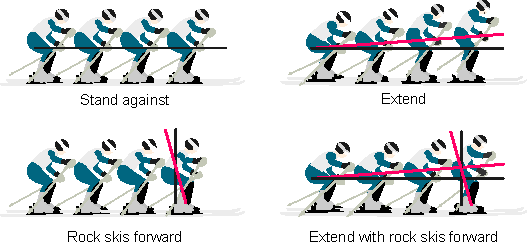
\includegraphics[width=1\linewidth]{figure/figure_introduction_strategies.pdf}
    \caption{Illustration of the strategies to improve reace times in flats in slalom}
    \label{fig: strategies}
\end{figure}



\section{What is the best way to teach these skills?}
The next question is whether insights from cognitive science can help coaches create more effective training. To ensure effective training, coaches generally have two main strategies for creating optimal learning situations at their disposal: designing learning problems for athletes and using effective teaching signals for instruction and feedback. In alpine skiing, skiers constantly face new slalom courses in races, requiring them to adapt their strategies and techniques. Therefore, their training should cover a wide variety of course scenarios to best prepare them to handle these diverse demands effectively. Given that coaches address this breadth of variation, should they also increase the frequency at which they expose their skiers to new learning problems? This is one of the questions we aim to test in this doctoral study. Another question is whether coaches can improve their use of instruction and feedback by selecting the most effective teaching signals.


\subsection{Can coaches improve skill learning by increasing the frequency at which they expose skiers to new learning problems?}
One learning effect that supports increasing the frequency at which coaches or teachers expose skiers to new learning problems is the contextual interference effect \cite{lee_contextual_2012, shea_contextual_1979, magill_review_1990}. This teaching strategy involves training learning problems (in our case courses) in a nonrepetitive sequence (that is, interleaved order), such as practicing learning problems A, B, and C in the order of BCA, ACB, or ABC, rather than a practice structure where problems are repeated in blocks (that is, blocked practice), such as AAA, BBB, or CCC. This nonsystematic training structure has been shown to be an effective teaching strategy for improving skill retention and transfer in various simple learning tasks \cite{tsutsui_contextual_1998, simon_metacognition_2001, shea_context_1983, shea_contextual_1979, tsay_signatures_2023}.

Two main explanations have been proposed to account for the contextual interference effect: the elaboration hypothesis \cite{shea_contextual_1979, shea_context_1983} and the reconstruction/forgetting hypothesis \cite{lee_can_1985, lee_locus_1983}. The elaboration hypothesis proposes that interleaved practices prompt individuals to process information more eloborately during acquisition, which enriches their understanding and problem solving techniques. This increased elaboration process enhances retention, which is not fully realized when practicing learning problems in a blocked order \cite{shea_contextual_1979, shea_context_1983}. In contrast, the reconstruction/forgetting hypothesis posits that increased problem switching provides more opportunities to forget task-relevant information held in working memory. This forgetting of task-relevant information forces the learner to reconstruct the action plan for every trial the learner revists the task. The repetitive process of abandoning and reconstructing action plans during interleaved practice contributes to better memory formation and thus increased retention \cite{lee_can_1985, lee_locus_1983}.

The contextual interference effect has not always succeeded in transferring to the learning of real-world skills, however \cite{wulf_principles_2002, brady_theoretical_1998, barreiros_contextual_2007, AMMAR2023100537, guadagnoli_challenge_2004}. This discrepancy can be understood through the challenge-point framework \cite{guadagnoli_challenge_2004} and recent extensions of it \cite{hodges_extended_2022}, where the effect of contextual interference is moderated by both the difficulty of the task and the skill level of the performer. In this framework, easy tasks can benefit from contextual interference to make the task more challenging, whereas difficult tasks are already challenging enough to serve as adequate learning stimuli on their own and are best learned without contextual interference initially. As the learner becomes more skilled, the learning process may benefit from increased contextual interference to improve the level of difficulty. In align with this prediction, studies have shown that beginners who learn skills when practice increases from blocked to interleaved practice learn better than those who use blocked or interleaved practice alone \cite{porter_systematically_2010, saemi_practicing_2012}. 

One prediction derived from the challenge point framework is that skilled athletes can benefit from interleaved practice to make training more challenging and therefore better. Consistent with this notion, \cite{hall_contextual_1994} found that skilled baseball players who practiced batting achieved better retention through interleaved practice than through blocked practice. In contrast, \cite{buszard_quantifying_2017} found no statistically significant differences in retention between tennis players learning to serve through interleaved practice and those using blocked practice. Instead, these researchers found evidence for improved transfer to new situations. Thus, it is not entirely clear whether contextual interference can be generalized to skilled performers. One idea is that contextual interference is more beneficial in open sports, where performers must constantly switch between different strategies to solve tasks, potentially making it important for alpine skiers \cite{farrow_chapter_2017, buszard_quantifying_2017}. An important aim of this study is to investigate whether the contextual interference effect can be used to improve the training of skilled performers. 

\subsection{Can coaches improve their instruction and feedback using reinforcement learning?}
Den andre treningsstrategien trenere kan bruke for å skape gode læringsbetingelser er gjennom gjennom teaching signalet de bruker for instruksjon og tilbakemeldinger. Although we exercise caution in generalizing and asserting that all coaches teach in a specific way, er det vanlig formen for teaching signal trenere bruker er instruksjonsbasert teaching \cite{williams_practice_2005, williams_effective_2023, hodges_modelling_2002}. In this approach, they offer performers a correct solution followed by corrective feedback. For instance, a ski coach may encourage the skier to take a shorter line around the gate and then further encourage the learner to shorten the line after a few trials. This teaching strategy can be likened to supervised learning in motor learning, where the difference between the desired strategy and the performer's movement outcome represents a teaching signal for skill improvement  \cite{jordan_forward_1992, wolpert_motor_2010, doya_complementary_2000}. Through practice, this teaching signal can bring the performer closer to executing what is assumed to be the correct choice. But is this teaching strategy truly the most effective approach for enabling learners to select and employ effective strategies? 

Supervised learning offers a promising approach for assisting learners in making informed strategy choices, yet it may also lead learners away from discovering the optimal strategy. First, the coach's advice may not be the optimal solution, as the strategy that coaches believes to be optimal does not always align with reality, even for the best-trained eye \cite{supej_impact_2019, cochrum_visual_2021}. Consequently, learners might be hindered to learn the best strategy when coaches opt for suboptimal strategies \cite{gray_plateaus_2017}. Worse, these learned suboptimal strategies might turn into habits that can be difficult to break \cite{popp_effect_2020}. Second, learners trained through supervised learning might also be constrained to adopting a single ('universal') strategy for all situations rather than acquiring a repertoire of strategies and discerning the most effective strategies for each specific scenario. Finally, it remains uncertain whether the prescriptive approach is the most effective teaching strategy for enabling performers to achieve long-lasting learning effects \cite{wulf_instructions_1997, hodges_role_1999, williams_practice_2005,williams_effective_2023}. 

Another, yet much less frequently adopted, teaching strategy to help learners learn to make good choices is through reinforcement learning \cite{sutton_reinforcement_2018}. The cornerstone of this approach is that the learner learns from evaluations instead of instruction, which occurs by using successes and failures of outcomes as teaching signals. That is, the performer learns the value of different strategies which allows them to finally pick the best solution, rather than being told the putatively correct solution to the problem. Specifically, these values are learned by comparing a given choice's outcomes with the choice's currently expected outcome. Outcomes that exceed or fall short of expectations result in errors in reward prediction, signaling that the learner must update their predictions to better anticipate future rewards following that action \cite{rescorla_theory_1972}. These reward prediction errors are then incorporated to form a new and better estimate of expected reward by updating expectations through a weighted running average. The computations underlying this form of value-learning of choices have been tremendously powerful in explaining human and animal learning \cite{waelti_dopamine_2001, schultz_neural_1997, pessiglione_dopamine-dependent_2006,lee_neural_2012, law_reinforcement_2009, tobler_human_2006} as well as training AI to perform complex tasks such as computer games starting from pixel inputs, only\cite{mnih_human-level_2015}. In addition, reinforcement learning has been shown to improve motor skill learning on simple tasks performed in the laboratory \cite{lior_shmuelof_overcoming_2012, abe_reward_2011, truong_error-based_2023, hasson_reinforcement_2015}. Based on this evidence, we ask whether reinforcement learning offers a better alternative for training learners to make better decisions about strategies than traditional supervised learning with a coach. 



\chapter{Aims}
The aim of this doctoral project was twofold. On the one hand, the project aimed to develop a better understanding of how to achieve better race times on flats in slalom and strategies to support this goal. In addition, the project aimed to understand the kinematic signatures of the "extend" (pumping) strategy by examining the kinematic changes after a training intervention on this strategy. On the other hand, this doctoral thesis aims to test whether learning theories from cognitive science can improve skill learning in sports through better problem-solving tasks and more effective teaching signals. The two overarching goals of this doctoral thesis are mutually important and have developed in parallel. Based on these goals, I have identified four research questions that the thesis aims to address:

\begin{itemize}
    \item Which strategies do skilled skiers perform best with on flat sections? (Study 2; not published as paper) 
    \item What are the kinematic changes resulting from a prolonged training intervention on the pumping strategy (or extend strategy)? (Study 1; Paper 2)
    \item How should coaches best distribute problem-solving tasks among skilled skiers? (Study 1; Paper 1)
    \item Which teaching signal is most effective for helping skiers learn to select effective strategies for skiing fast on flat sections?  (Study 2; Paper 3)
\end{itemize}












\chapter{Method}


\section{Study overview}
The thesis is based on data from two learning experiments, referred to as Study \RNum{1}  and Study \RNum{2}. Study \RNum{1} has resulted in Paper \RNum{1} og Paper \RNum{2}. Study \RNum{2} has resulted in Paper \RNum{3}. Additionally, we used data from this learning experiment for an additional analysis reported in Section \ref{results_strategies}.

Study \RNum{1} was designed to test whether frequent task switching can enhance learning. This experiment spanned eight days, starting with a baseline test on day one, followed by three days of training intervention. This training intervention contrasted two training groups learning to pump on flat slopes in slalom: an interleaved training group, which practiced pumping on three slalom courses each day in interleaved order (ensuring skiers never repeated the same slope consecutively), and a blocked training group, which practiced pumping on one slalom course each day (with the order counterbalanced across skiers). After the training period, the skiers had a three-day break without skiing. On the third day, they completed a retention test. This study resulted in Paper \RNum{1}, which reports the learning effects between the two learning groups. Additionally, we collected positional data from the skiers using a local positioning system during the baseline and retention to study the kinematic changes due to the intervention. This analysis is reported in Paper \RNum{2}. 

\begin{figure}
    \centering
    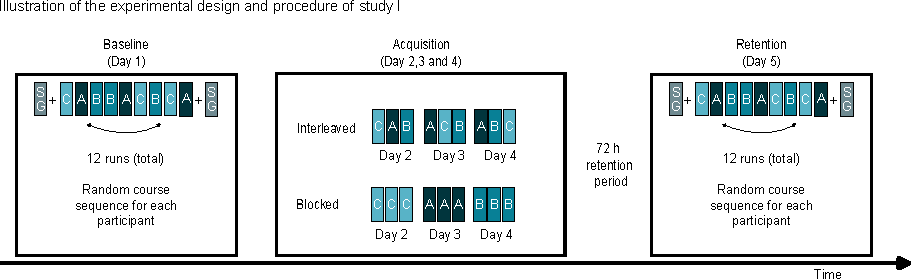
\includegraphics[width=1\linewidth]{figure/figure_methods_CIdesign.pdf}
    \caption[Illustration of the experimental design and procedure of Study \RNum{1}]{Illustration of the experimental design and procedure of Study \RNum{1}. On baseline (day 1), all skiers performed a baseline test that consisted of three runs in each of the three slalom courses A, B and C  (see Fig.\ref{fig:slalomcourses}), performed in an interleaved order, plus a straight gliding (SG) before and after these runs. The skiers were then assigned to either the interleaved or the blocked learning groups. Skiers in the interleaved group skied all courses each day, executed in an interleaved order under the condition that no more than two runs in the same course would occur consecutively. Skiers in the blocked group performed all runs on a single course (that is, course A, B or C) in a given session. The order in which the skiers performed the course was counterbalanced across skiers. After a retention interval of 72 h, the skiers returned to complete a retention test that was similar to the baseline test. The figure is adapted based on the illustration figure in \cite{magelssen_is_2022}.}
    \label{fig: ci_illustration}
\end{figure}


Study \RNum{2} was designed to identify the most effective teaching signal for helping skilled performers learn strategy selection to enhance performance. This learning experiment spanned three days, beginning with a baseline test on day 1. This baseline test was followed by a training intervention (acquisition) consisting of three training sessions. The intervention contrasted reinforcement learning with two supervised learning groups as teaching signals. In the reinforcement learning group, the skiers learned to select optimal strategies by seeing their times to inform their next strategy choice. Conversely, in the supervised learning groups, the coaches selected strategies for the skiers. In the supervised (target skill) learning group, we educated experienced coaches on the theoretically optimal strategy and instructed them to select this strategy for the skiers and give them feedback on this strategy after every trial. In the supervised (free choice) learning group, we recruited two coaches from each group of the tested ski teams to select a strategy that they believed would make the skier faster. Before allowing the skiers (reinforcement learning) or the coaches (supervised learning) to freely choose strategies, we conducted a forced exploration session where all participants tested every strategy. On day 3, the skiers performed a retention test and a transfer test, independently select strategies. This study resulted in Paper \RNum{3}, which reports the learning effects of the two teaching signals on strategy selection. Additionally, we used data from the forced exploration session to analyze and estimate which strategies yielded the best performance for the skiers. Denne analysen er også gjort Paper\RNum{3}, men vi har gjort en ekstra analyse som vi har rapportert her. 
\begin{figure}[H]
\centering
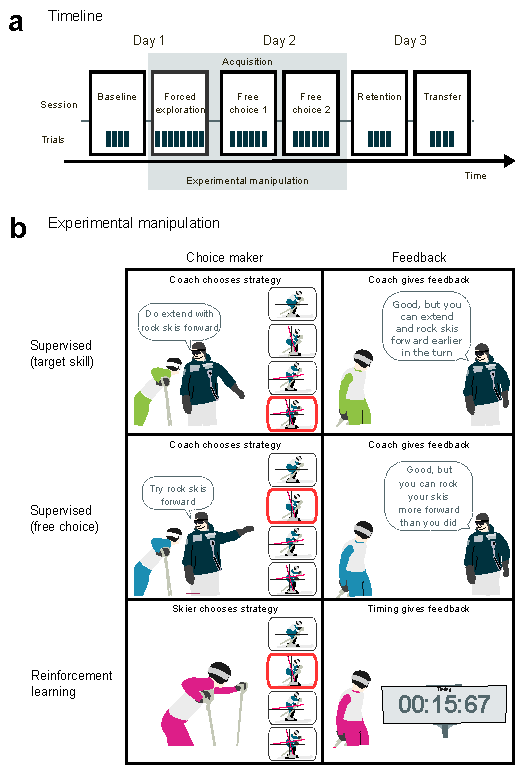
\includegraphics{figure_method_experiment.pdf}
\caption[Illustration of the experimental design and procedure of Study \RNum{2}]{Illustration of the experimental design and procedure of Study \RNum{2}. \textbf{a.} Timeline of the three-day learning experiment. During the baseline session, the skiers raced a slalom course in the shortest time possible without receiving race time feedback. The skiers were then assigned to one of three learning groups (see b). In their assigned group, the skiers underwent three acquisition sessions, comprising one forced exploration session (skiers performed all strategies) and two free choice sessions (skiers or coaches could choose strategies themselves). On the last day, skiers completed a retention and transfer test where they could pick strategies themselves, again without receiving race time feedback. \textbf{b.} Illustration of the learning groups in the study. The supervised (target skill) learning group involved coaches consistently choosing the theoretically best strategy (except during forced exploration), while in the supervised (free choice) learning group coaches freely selected strategies. The skiers in both of these learning groups received feedback on strategy execution from their assigned coach, while the skiers in the reinforcement learning group independently selected strategies and received feedback from the timing system to facilitate value learning of each strategy.}\label{fig: rlillustration}
\end{figure}


\section{Setup}
All studies were conducted in the indoor ski hall, SNØ, located in Oslo, Norway (\url{https://snooslo.no/}). In this ski hall, we used the upper part of the race hill, which is a long flat section with two small rollers. The snow of this flat section was watered before testing each group of skiers to ensure uniform and fair conditions for all skiers. 

\begin{figure}
    \centering
    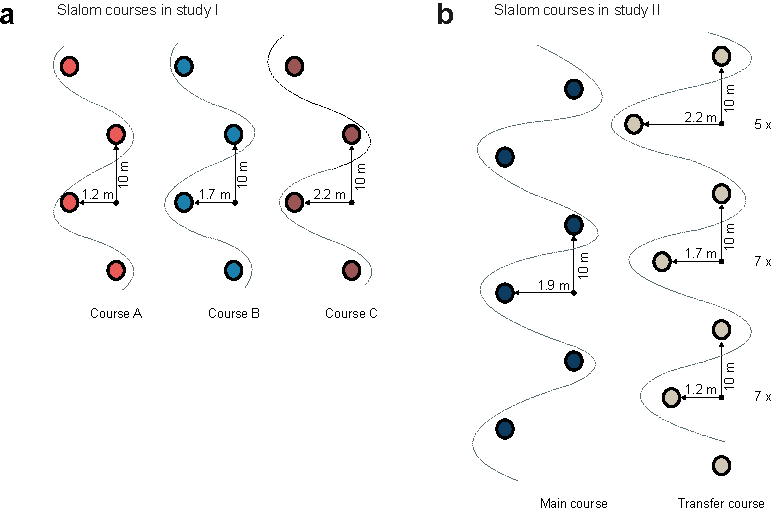
\includegraphics[width=1\linewidth]{figure/figure_methods_courses2.pdf}
    \caption[Illustrations of the slalom courses used in the studies in \RNum{1} and \RNum{2}]{Illustrations of the slalom courses used in the studies. \textbf{a.} The three slalom courses used in Study \RNum{1} to probe the contextual interference effect. Course A had the smallest gate offset whereas Course C had the largest offset. \textbf{b.} The two slalom courses used in Study \RNum{2} to compare reinforcement learning to supervised learning. The main slalom course was a rhythmic course deployed in all sessions except for the transfer session. The course setting for the transfer session involved a progression in gate offset, starting with the largest offset and ending with the smallest offset.}
    \label{fig:slalomcourses}
\end{figure}

In study \RNum{1}, we set up three slalom courses to test the contextual interference effect. These courses required skiers to execute pumping movements with different timings and amplitudes for effective performance. All three courses had a vertical gate distance of 10 meters due to space constraints, forcing parallel setup. However, the courses had varying offsets: 1.2 meters for Course A, 1.7 meters for Course B, and 2.2 meters for Course C. These specific gate offsets were chosen to create diverse pumping demands without making it impossible to pump. Fig. 

In study 2, we set up two slalom courses to test. The main slalom course was used in all sessions except the transfer test and featured a 10-meter distance and a 1.9-meter offset. The transfer test assessed skiers' ability to transfer learning to a more realistic alpine race course. This test course included a progression in gate offset: five gates at 2.2 meters, seven gates at 1.7 meters, and seven gates at 1.2 meters. 

In both studies, we used stubbies (short gates) instead of long gates to minimize energy dissipation upon hitting the gate\cite{minetti_biomechanics_2018}. Using stubbies allowed skiers to focus better on skill execution of the strategy without the distraction of clearing the gate, which could hinder learning. In addition, this approach minimized hole creation that occurs when a long gate is forcefully slammed into the ground. 

We adopted the same standardized start procedure in both studies. The involved setting the start gate 20 meters before the first gate. Here, skiers were instructed to place their toe bindings behind the starting gate. Upon receiving the clearance signal, skiers were to place their skis parallel, lift the poles from the ground, and glide out of the start gate without using poling or skating to generate propulsion. Timing was recorded using a wireless photocell timing system (HC Timing wiNode and wiTimer; Oslo, Norway), starting when the skier crossed the first photocell pair situated 10 meters below the starting gate. (See https://osf.io/9numq for a supplementary video illustrating the starting procedure and setup).


\section{Participants}
Our target population for making inferential claims was skilled alpine skiers worldwide. Therefore, we recruited only skiers aged 15 and older, marking the entry age for participating in Federation Internationale de Ski (FIS) races. We chose skiers aged 15 years and older to ensure that they could handle the icy snow conditions we prepared in the ski hall and had the basic skills necessary to learn the strategies we developed. Beyond these criteria, we deliberately recruited skiers with diverse skill levels—from skilled junior ski academy skiers to Olympic skiers—to enhance the generalizability of our findings.

Our sample size approach in both studies was to recruit as many skiers as possible during the available testing window, and was justified by the 'resource constraints' and the 'whole population' criteria \cite{lakens_sample_2022}. First, the relatively small and geographically dispersed population of skilled alpine skiers limits the number of available participants.  Second, coaches and skiers must be willing to participate in the intervention. For coaches and skiers at this level to show this willingness, they must be convinced that the intervention will benefit the skiers' development, as it typically replaces the skiers' regular training due to their already high training volumes. Finally, the narrow testing window, typically in the spring and summer, coincides with the indoor skiing training periods for many ski teams, leading to a high demand for training lanes. These combined factors make it challenging to recruit a large number of participants and to reach a specific benchmark.  

In Study 1, we successfully recruited 66 skilled alpine skiers (31 females) from Norway, with a mean age of 17 years (SD = 2.7). Of these, 51 skiers attended ski academies and had either already earned International Ski Federation (FIS) points or were about to do so in the upcoming season. Twelve skiers competed at the club level in age-specific categories for those aged 14 to 16 (but with the necessary skill level), while three skiers were elite skiers outside the national team preparing for the next season. Unfortunately, due to COVID-19, 12 of these 66 skiers were quarantined and unable to participate in the retention session. We did not ask the first groups of the tested ski teams to report their FIS points on slalom, resulting in a lack of FIS points and world ranking data for these skiers. 

Study 2 involved a smaller sample (n=18) from the larger pool of skiers in Study 1 (n=66), where we recorded the skiers' positions using a local positioning system in the upper section of the course. The smaller sample included 18 alpine skiers (mean age = 16.7 years, SD = 1.1; 7 females, 11 males) from three ski academies. Except for three skiers, all participants had previously competed in FIS races, with recorded FIS points in slalom (M = 115, SD = 31). However, these FIS points may not accurately reflect their skill levels due to the pandemic-related challenges in organizing races, which limited opportunities to accumulate points.

In Study 3, we successfully recruited 98 alpine skiers from Norway and Sweden (mean age = 18.1 years, SD = 2; 40 females, 58 males). Two skiers were excluded from the analysis due to injury prior to the study (n=1) or sickness (n=1), resulting in 96 skiers who completed the study and were included in the analysis. The tested groups of skiers included five ski academies, three senior development teams, and two national ski teams. The skiers were generally highly skilled, with mean FIS points in slalom 55.4 (SD=32). Their median world rank was 605, though there was considerable variability (Q1 = 248, Q3 = 1390.5). A smaller subset of skiers (n = 13) were not world-ranked, as they had yet to compete in internationally sanctioned races necessary for calculating FIS points and rankings. Before data collection for this study, we set the minimum sample size to 80 skiers, which we deemed appropriate for this context. Prior to data collection, we conducted power simulations for sample sizes of 80, 100, and 120 skiers. These simulations revealed powers of 0.60, 0.75, and 0.80, respectively, for the smallest effect size of interest (0.3 second difference between groups) (\url{https://osf.io/c4t28}). 


\section{Design and procedure}

\subsection{Study 1}
In Study 1, we employed a between-subjects design and allocated skiers to either a blocked or interleaved learning group. The experiment began with a baseline test consisting of nine trials (three trials on each of courses A, B, and C), where skiers skied as quickly as possible without receiving time feedback. The trials in these courses were distributed randomly to each skier under the condition that the skier did not perform no more than two consecutive runs on the same course. In addition, the skiers performed a straight gliding task on a dedicated lane before, midway (randomly assigned), and after the nine trials.

After the baseline test, we used a randomized-blocked design to allocate skiers into either the blocked or interleaved learning group based on their baseline test times. Specifically, we extracted each skier's best run from the baseline on each course and divided it by the average of the straight gliding runs from the baseline. Skiers were then ranked from fastest to slowest and paired in ascending order, and each consecutive pair was randomly assigned to either the interleaved or blocked group.

Immediately after the baseline test on day one, skiers attended a workshop where we explained the mechanical principles of the pumping technique and presented quantitative evidence supporting this strategy. Skiers then completed three training sessions over three days, with each session including 15 runs: 12 runs on the three courses and three straight-gliding runs. The interleaved group skied all three courses each day in a randomized interleaved order, ensuring no more than two consecutive runs on the same course. The blocked group performed all their runs on one course (A, B, or C) per day, with the course order counterbalanced across participants. 

Three days (72 hours) after the last training session, the skiers returned for a retention test, consisting of 12 runs (three runs on each of the three slalom courses and three straight-gliding runs). The order of the runs in the courses was scheduled in a semirandom order, with the condition that no more than two consecutive runs could be performed in the same course. As in the baseline test, the skiers performed a straight gliding task on a dedicated lane before, midway (randomly assigned), and after the nine trials. The skiers were instructed to ski as fast as possible but did not receive any performance feedback during the posttest. This design allowed us to compare the effects of blocked versus interleaved practices on the learning and performance of the pumping strategy. 


 \subsection{Study 2}
In Study 2, we employed a between-subjects design and framed the task of learning to choose effective strategies as a multiarmed bandit problem\cite{sutton_reinforcement_2018}. Here, the options (or bandits) that the skiers needed to learn and select to ski as quickly as possible were the four technical strategies detailed in section \ref{introduction: strategies}.

To test which teaching signals most effectively drive this learning process, we allocated skiers into one of three learning groups. In the supervised (free choice) learning group, skiers were told by their coaches which strategy to use, either the one they believed to be the best or most appropriate for the skier. This learning group represents the conventional teaching strategy in alpine skiing. We complemented this learning group with a supervised (target skill) learning group, where coaches instructed skiers to select the strategy that we defined as the theoretically best strategy (that is, "extend with rock skis forward") based on mechanics and field observations of elite skiers (see section \ref{introduction: strategies}. Since the skiers were instructed to use the theoretical optimal strategy, this learning group served as a benchmark for the upper limit of performance achievable through optimal strategy choices. In both of these supervised learning groups, the coaches saw the skiers’ race times but did not communicate them to the skiiers. We compared these two learning groups to a reinforcement learning group where the skiers learned the values of the strategies by trying a strategy and learning from evaluations (that is, race times) instead of from a coach.
%In the supervised (target skill) learning group, the skiers were instructed by a coach to choose the theoretically best strategy (that is, extend with rock skis forward) and received feedback on their execution of this strategy after every trial. For this learning group, we engaged highly experienced ski coaches to ensure credibility in promoting this strategy, and these coaches were educated by us before the data collection. To the skiers, these coaches told that the 'extend with rock skis forward’ strategy was the most effective strategy for skiing fast on flat terrain in slalom, citing theory and quantitive evidence from research literature in alpine skiing mechanics \cite{reid_kinematic_2010, mote_accelerations_1983, lind_physics_2013, lemaster_skiers_1999, lemaster_ultimate_2010}. In the supervised (free choice) learning group, the skiers were assigned to one of two coaches selected from the ski team undergoing testing. These coaches were instructed to maximize their assigned group of skiers' performance in the slalom course by choosing one of the four strategies for each trial. Although the coaches in these two supervised learning groups had access to the skiers’ data after each trial, they were not allowed to share the times with the skiers. In contrast, the reinforcement learning group learned the value of these strategies themselves by observing the times for a chosen strategy after every trial to guide their strategy choices, with the aim to select the best strategy. This group was not assigned a coach but a person to communicate with the skiers, record their choices, and encourage them to ski quickly to prevent boredom effects. See the original paper for more information.

The learning experiment began with a baseline session consisting of four runs through the slalom course (main course in Fig. \ref{fig:slalomcourses}) plus one straight gliding run where the skiers skied straight down the course section in a dedicated lane. Before these four runs and straight gliding, the skiers completed two warm-up runs: one as free skiing and one as a warm-up in the course, where they received instructions and feedback on their starting procedure. 

After the baseline, we assigned the skiers to three learning groups: supervised (target skill) learning, supervised (free choice) learning, and reinforcement learning. For this assignment, we used a randomized blocked approach to account for preexisting differences among the skiers \cite{maxwell_designing_2017}. Specifically, we computed each skier’s average performance across the four baseline trials and ranked them accordingly. We then created blocks, with sizes corresponding to the three learning groups, and assigned the skiers to these predefined blocks based on their rankings. Finally, we randomly allocated the skiers within each block to the different learning groups. Meanwhile, the skiers had a 60-minute break in a warm zone. 

The learning groups participated in sessions at different times to prevent treatment
diffusion \cite{maxwell_designing_2017}. Since the ski group consisted of teams that regularly trained and lived together during data collection, they were instructed to keep session information private. To complete the learning experiment within the ski hall's opening hours, the two supervised learning groups underwent training simultaneously. We arranged coach stations in the finishing area with space and vision dividers to prevent information leakage between coaches. Additionally, a Python script was used to fetch race times from the timing system, which were filtered for each coach and transmitted to the respective station so that each coach could only see their own skiers' times (SEE). The learning group that begun traing after the learning group assignment (reinforcement learning versus supervised learning) was randomized and counterbalanced across the ski teams tested. 

During the first session following the learning group assignment, we engaged the skiers in forced exploration. Here, we began by gathering the skiers within each learning group and followed by introducing them to the four strategies identified to enhance racing times on flat slopes in slalom. Each strategy was detailed with illustrative drawings and word explanations, as outlined in (SJEKK). To ensure understanding, skiers participated in two short familiarization trials for each strategy or continued until their execution met our standards. After reviewing the strategies, we asked the skiers and the coaches in the supervised (free choice) learning group to rank the strategies (1=best; 4=worst) based on their perceived effectiveness in improving race times on flat sections of a slalom course. We explicitly instructed the coaches and skiers not to discuss the strategies with each other during the instruction and ranking process. Notably, the same instructor conducted all learning sessions within the tested ski group. Following this review, the skiers performed eight trials on the slalom course, testing all strategies with two trials per strategy. Strategies were randomly assigned, ensuring that the first and last four trials included all strategies. During this session, the reinforcement learning group received feedback on their timing, while the coach provided feedback in the supervised learning groups.

On the second day, the skiers completed two free choice sessions, each comprising a total of 6 trials in the same slalom courses that were used for the baseline testing the day before (that is, the main course). Prior to the 6 free choice trials, the skiers performed one warm-up free skiing run and one warm-up run in the slalom course. In these sessions, the supervised (target skill) learning group consistently selected the theoretically best strategy (that is, 'extend with rock skis forward'). Conversely, in the supervised (free choice) learning group and the reinforcement learning group, the coach and the skiers, respectively, had the autonomy to choose the skiing strategy for each run. After each session, coaches (except supervised target skills) and skiers were asked to re-evaluate and rank the strategies.

On the third and last day, the skiers performed a retention test and a transfer test to assess the effect of the training approaches on learning and performance. The retention test was performed in the same course as the baseline and acquisition sessions, whereas the transfer test was performed in the transfer course and involved a progression in gate offset from start to finish. Since the transfer test was a new course, we allowed the skiers to inspect the course before the test. The retention and transfer tests were conducted with the three learning groups together. None of the learning groups received any feedback from coaches or time during these tests. After each test, the skiers were asked to rank the strategies.








%Læringseksperimentet begynte med en baseline som bestod av fire runder i slalåmløypen (main course in Fig. \ref{fig:slalomcourses}), pluss en straightgliding runde der utøverne kjørte rett ned løypeseksjonen i en egen dedikert bane for dette. Før utøverne gjennomførte disse fire rundene og straight glidingen gjennomførte de to oppvarmingsrunde: en gjennomført som frikjøring og som gjennomført som oppvarming i løypen, der de fikk instruksjoner og tilbakemelding på utførelsen av startprosedyren. 

%Etter dette allokerte vi utøverne i tre læringsgrupper supervised (target skill) learning, supervised (free choice) learning and reinforcement learning. For denne oppgaven brukte vi en randomisert blocked approach for å ta hensyn til preeksisterende forskjeller mellom utøvere. Specifically, we computed each skier’s average across the four trials at baseline and ranked them accordingly. We then created \textit{n} blocks with block sizes corresponding to our three learning groups for the entire list of skiers and assigned these skiers to these predefined blocks. Finally, we randomly allocated the skiers to the different learning groups within each block (Fig. \ref{fig:experiment}b). I mellomtiden hadde utøverne en pause på 60 minutter i varm sone. 





\section{Measures and analysis}
De ulike målene og forskningspørsmålet har favnet nokså bredt. Derfor har jeg valgt å dele inn measures og analyse etter hva som er formålet med de enkelte studiene. 


\subsection{Paper 1}
I Paper \RNum{1} var målet å teste om kontekstuell interferens effekten på gode skikjørere. Her regnet vi prestasjon som tidsforskjellen mellom tiden i løypen og gjennomsnittet av rundene hvor utøverne gjennomførte straight gliding. 


\subsection{Paper 2}
I Paper \RNum{2} var målet å forsøke å forklare forbedringer i renntidene fra Studie \RNum{1}. For å få innsikt i dette monitored vi skiers using a local positioning system in a five gate long section in the middle of the course during the baseline and retention sessions. Opprinnelig var det opprinnelige opptaksområder betydelige lenger, men på grunn av utfordringer med data kvaliteten i det øverste området av sekvensen (der nodene kom for tett på veggene i skihallen) måtte vi korte ned området. 

\subsection{Paper 3}
In Paper \RNum{3} (basert på Studie \RNum{2}) ønsket vi å teste om reinforcement learning forbedret sine renntider mer under trening (acquisition) og presterte bedre under retention og transfer enn supervised (free choice) learning, men også å sammenligne opp mot supervised (target skill) learning som var på benchmark gruppe for optimal prestasjon gjennom optimale valg av strategier. To account for these multilevel data structures, we leveraged linear mixed-effects models. To model random effects, we adopted a design-driven approach \cite{barr_random_2013, barr_learning_2021}, where we sought to account for all nonindependence introduced by repeated sampling from the same ski group and skier. We deployed classical frequentist statistics and fitted these models with the lme4 package \cite{bates_fitting_2015} in the R \cite{r_core_team_r_2022} programming language. We used a simple coding scheme for our predictors where the intercepts represent the estimated mean of the cell means and the contrasts represent the estimated difference with respect to the reference level, which we set for reinforcement learning. Two-tailed p values and degrees of freedom for each model were derived using the lmerTest package \cite{kuznetsova_lmertest_2017} via the Satterthwaite approximation method. Alpha was set to 0.05 for all test statistics.




These race times were analyzed using linear mixed-effect regression models. Initially, we planned to normalize the racing times by expressing the racing times as the difference from the straight-gliding time performed at the beginning of every session (like we did in Study \RNum{1}). However, practical considerations led us to deviate from this approach. This change was necessary because we had to flip or shift the course after each day to ensure snow conditions with the least damage. Unfortunately, these adjustments made maintaining a clean, straight-gliding lane difficult since the straight gliding lane crossed many areas with damage to the snow surface (holes) from the previous course set (see Supplementary Methods C for an image of these holes). Collisions with these holes affected the race time, adding noise to the results. Therefore, we used a more conservative approach and analyzed the raw racing times instead of analyzing the normalized racing times.

For the acquisition session, we modeled race time using Session (forced exploration, free choice 1, free choice 2) and Learning group (reinforcement learning, supervised: free choice learning, supervised: target skill learning), and their interactions, as predictors. For retention and transfer, we modeled race times at these sessions, with learning group added as a predictor. In addition, we used the average performance for each skier on the baseline test as a predictor to improve estimate precision and adjust for any group differences at baseline testing. 

To model the effect and development of the strategies we broke the analysis up into different sub-models. One analysis focused on differences in the strategies and groups regarding Forced Exploration, where all participants had completed all strategies. Another analysis examined the transition from Forced Exploration to retention for both supervised (free choice) and reinforcement learning. The final model investigated the development between groups specifically for the "extend with rock skis forward" strategy. Session was coded as a continuous variable in all models. 

I artikkelen har vi også forsøkt å forklare disse tidene, men har valgt å ikke presentere disse analysene i denne thesis og dermed også ikke presentert dem her. 










Due to the hierarchical structure of the data, our general statistical strategy relies on multilevel modeling. At the first level, each skier performed multiple trials during each session. At the second level, each skier was nested within groups of ski teams that performed the experiment together. To account for these multilevel data structures, we leveraged linear mixed-effects models. To model random effects, we adopted a design-driven approach \cite{barr_random_2013, barr_learning_2021}, where we sought to account for all nonindependence introduced by repeated sampling from the same ski group and skier. We deployed classical frequentist statistics and fitted these models with the lme4 package \cite{bates_fitting_2015} in the R \cite{r_core_team_r_2022} programming language. We used a simple coding scheme for our predictors where the intercepts represent the estimated mean of the cell means and the contrasts represent the estimated difference with respect to the reference level, which we set for reinforcement learning. Two-tailed p values and degrees of freedom for each model were derived using the lmerTest package \cite{kuznetsova_lmertest_2017} via the Satterthwaite approximation method. Alpha was set to 0.05 for all test statistics.































\chapter{Results and discussion}
I have structured the results as follows: First, I present results that answer "What can skilled skiers do to ski faster on flat sections in slalom?". In this section, I present data from the skiers' race times on the different strategies during Study \RNum{2} and velocity and path length data from the local positioning data from Study \RNum{1}. Then, I present results that answer "How should we train skiers to ski faster on flat sections in slalom?". Here, I first present the results from Study \RNum{1}, which tested whether the contextual interference effect can be leveraged to improve skill learning by creating learning problems for skiers.  . Finally, I present the results from Study \RNum{2}, which tested which teaching signal that is most effective in helping skiers learn the values of strategies to make them pick the best one.  

\section{What can skilled skiers do to ski faster on flat sections in slalom?}


\subsection{Which strategies did the skiers perform best with?}\label{results_strategies}
We begin by assessing which of the four strategies—"stand against", "rock skis forward", "extend", and "extend with rock skis forward—yielded the best average race times for these skilled skiers. To compare these strategies, we collected the race times from the forced exploration session from Study \RNum{2}, where the skiers in all three learning groups tested all strategies. Since we accounted for practice order effects during this testing, by randomly assigning the test order of the strategies to each skier (under the condition that the first and last four trials included all four strategies), we could use these times to compare the effectiveness of the strategies. 

To this end, we employed a Bayesian modeling approach to estimate the expected differences between the strategies (Supplementary Table \ref{study3:estimateddifferencebetweenstrategies}). This analysis revealed that skiers on average achieved their best race times using the 'extend with rock skis forward' strategy (16.66 s, 95\% credible interval (CI) = 16.54, 16.77). This strategy was only marginally better than the 'extend' strategy, with a mean difference of just 0.02 s (95\% CI = -0.02, 0.06).  We found a more substantial expected time loss when skiers switched from the 'extend' strategy to the 'rock skis forward' strategy, with an average loss of 0.21 s (95\% CI = 0.16, 0.25). Finally, if the skiers switched from the "rock skis forward" strategy to the "stand against" strategy, the expected time loss was 0.2 s (95\% CI = 0.15, 0.25). Therefore, the strategies skiers used exerted a great impact on the skiers' race times. 

These results show that just making clean, carved turns and resisting the centripetal forces during a turn using the "stand against" strategy is insufficient for achieving fast race times on flat terrain in slalom. Instead, the active movements of the skiers were crucial for achieving fast race times on flats. When the skiers actively "rocked their skis forward", they improved their race time greatly compared to "stand against" only. This finding aligns well with prior findings in slalom skiing that reported a strong correlation between fore and aft movements and energy dissipation, such that more fore movements were associated with greater energy dissipation \cite{reid_turn_2009, reid_kinematic_2010}. Furthermore, studies have shown that faster skiers have a greater range of fore/aft motion and spend a larger portion of the turn skiing with their weight shifted back after gate passage than slower skiers \cite{tjorhom_beskrivelse_2007, reid_kinematic_2010}. Our results extend these findings and provide experimental evidence that "rock skis forward" can be an effective strategy for improving race times on flat terrain in slalom.

However, the 'rock skis forward' strategy resulted in much slower times than did the 'extend' strategy. Predictions from the Lind and Sanders model \cite{lind_physics_2004} indicate that extending the center of mass closer to the axis of rotation during a turn from a laterally inclined position should significantly improve the race time. Without motion capture data, we cannot assess the extent to which skiers extended and the resulting increase in kinetic energy. Nonetheless, the results suggest that skiers' extension movements play a crucial role in slalom performance, contrary to previous beliefs \cite{supej_differential_2008, supej_doba_2001}.

Finally, we found that "extend with rock skis forward" on average was the best strategy. This finding aligns with previous simulations suggesting that this strategy is most effective when skiers pump over rollers \cite{mote_accelerations_1983} and that it can be transferred to skiers executing a turn \cite{reid_kinematic_2010}. However, it is important to emphasize that "extend with rock skis forward" only was marginally better than the "extend" strategy alone. One reason for the limited improvement achieved by adding "rock skis forward" to the "extend" strategy might be that rocking the skis forward during the turn compromised how much the skier could extend toward the turn's axis of rotation. For instance, extensive extension could be challenging if the skier's center of mass was located at the tail of the skis. This issue should be further investigated in future analyses.

One limitation of these timing analyses is that we do not have precise knowledge of how much the skiers moved when executing the strategies or how these strategies affected the mechanical energy during a turn. Therefore, we cannot comment on the skiers' actual execution or the energy mechanics behind each strategy. Future studies should incorporate motion capture to address this gap in understanding.


\begin{figure}[H]
\centering
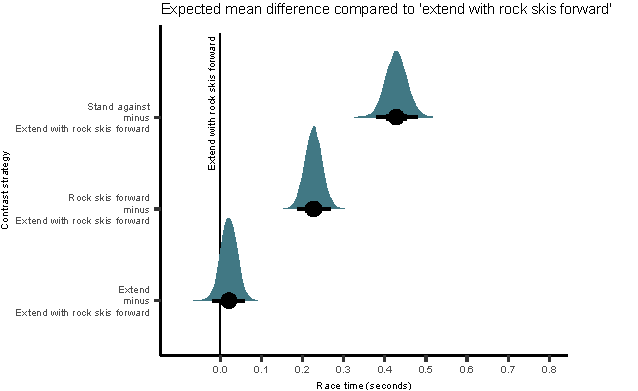
\includegraphics{figure/figure_results_Q1_strategies_2.pdf}
\caption[Expected differences in means between strategies compared to 'extend with rock skis forward']{Expected differences in means compared to 'extend with rock skis forward' (that is, the theoretical best strategy). The circle represents the point estimates whereas the shaded distribution represents the expected posterior of the mean differences from the model.}
\label{fig:q1_strategieseffect}
\end{figure}



\subsection{The kinematic changes following a training intervention on the pumping ("extend") strategy}
From the previous section, we learned that the 'extend' strategy was the second most effective strategy, only marginally surpassed by the 'extend with rock skis forward' strategy. In Study \RNum{1}, we found that skiers significantly improved their race times after a three-day training intervention focused solely on the 'extend' strategy. Our next aim was to examine the kinematic changes that occurred during this intervention to better understand what the skiers learned or did differently. In effect, this knowledge can help us acquire a better understanding of how this strategy exerts an influence on skiing. Since race time in alpine skiing depends on speed and path length, these kinematic changes could manifest as alterations in either speed or path length. We investigated which of these changes were most consistent with the data and whether the kinematic changes aligned with the mechanical theory of pumping. To explore these accounts, we used recording data from a small segment of the slalom course and a subset of skiers (18 out of 66) for whom we had set up a local positioning system in the upper section of the slalom course. This allowed us to quantify both path length and instantaneous speed.

If the pumping mechanism drove the skiers' improvement in race time, we would expect skiers to increase their speed at or immediately after gate passage, at the time when the extension movement occurs. Fig. \ref{fig:lps_speed}a shows the speed profiles for the local positioning system section during baseline and retention. We first describe the average speed trend at baseline and then the contrast between baseline and retention.

In the baseline test, the skiers’ speed decreased for each gate in the local positioning system section compared to their speed during straight gliding, except for a slight speed increase of 0.05 m/s (95\% CI[-0.08, 0.17]) from gate 1 to gate 2. In the other gate sections, the speeds decreased on average by -0.06 m/s (95\% CI[-0.19, 0.07]) from gate 2 to gate 3 and by -0.12 m/s (95\% CI[-0.25, 0]) from gate 3 to gate 4 compared to straight gliding times. We report only the comparisons at the gates because the gates mark a fixed reference point. After the training intervention, the skiers increased their entry speed into the local positioning section (gate 1) by an average of 0.24 m/s (95\% CI [0.19, 0.29]) compared to the baseline speed. From this gate, the skiers tended to increase their speed throughout the section. Specifically, the skiers increased their speed on average by 0.07 m/s (95\%CI [0.01, 0.12]) from gate 1 to gate 2, followed by a slight decrease of -0.02 m/s (95\%CI [-0.05, 0.02]) from gate 2 to gate 3. Subsequently, the speed of the skiers increased again by 0.1 m/s (95\% CI[0.06, 0.14]) from gate 3 to gate 4. Therefore, the speed of the skiers increased almost incrementally from gate to gate. In addition, the speed profiles appeared wavier, as depicted in Figure \ref{fig:lps_speed}b. In general, the pattern of these waveforms was that skiers increased their speed after gate passage and continued to rise until the skiers were approximately midway between two gates. After that, the speed decreased to the gate before it rose again. As such, the speed profile changed massively from baseline to retention. 

\begin{figure}
    \centering
    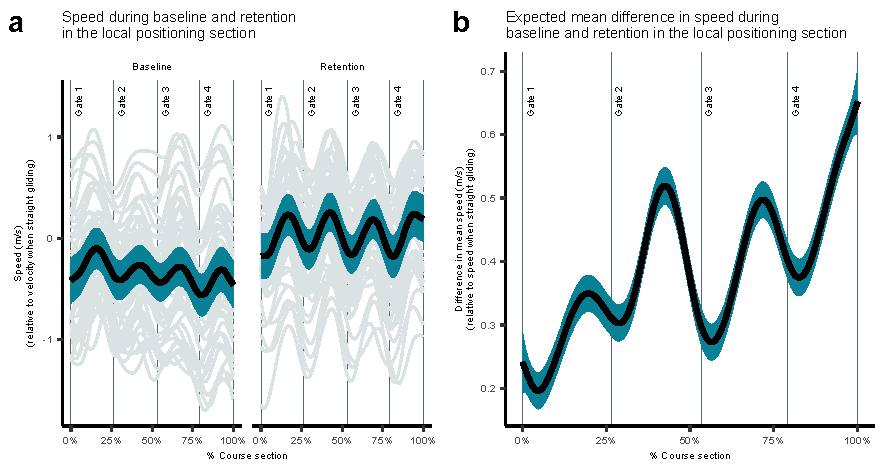
\includegraphics[width=1\linewidth]{figure/figure_speed_2.pdf}
    \caption[Speed in the local positioning system section from Study \RNum{1}]{Speed in the local positioning system section. \textbf{a.} Estimated speed during baseline and retention for the local positioning section. \textbf{b.} Estimated differences (contrast) between baseline and retention for the local positioning section. The black lines denote the expected mean or differences in mean, with the shaded area representing their 95\% credible interval (CI). Each gray line represents one run trial by a skier.}
    \label{fig:lps_speed}
\end{figure}


Next, we analyzed the path length, for which we did not expect would undergo big changes based on the recording system we used. At the baseline test, we found that the total path length from gate 1 to gate 2 was 10.00 m (95\% CI[9.97, 10.10]), 10.7 m (95\% CI[10.70, 10.80]) from gate 2 to gate 3, and 10.10 m (95\% CI[10.10, 10.10]) from gate 3 to gate 4, while it was 8.19 m (95\% CI[8.15, 8.23]) from gate 4 to the end of the section. Notably, the reason for the lower estimate from gate 4 to the end is that this section was shorter than the other gate sections because the section ended before gate 5. Fig. \ref{fig:lps_path}a shows the total path length during each gate in the local positioning system section. Overall, we found no clear systematic differences in path length from baseline to retention across the gates. Surprisingly, the expected mean difference was 0.17 m (95\% CI[0.06, 0.28]) longer from gate 1 to gate 2 in retention. This expected mean difference did not overlap with the baseline estimate. Conversely, the expected mean difference overlapped considerably between baseline and retention for gate 2 to gate 3 (-0.02 m, 95\% CI[-0.14, 0.10]) and for gate 3 to gate 4 (0.02 m, 95\% CI[-0.02, 0.06]). In contrast, we observed an increased path length in retention from gate 4 to the end of the section (0.08 m, 95\%CI[0.04, 0.13]). In summary, we found changes in path length for some gate sections, while others showed minor differences. The general trend was that the skiers skied a longer path length during retention than at baseline. Fig. \ref{fig:lps_path}b shows the expected mean difference in total path length for each gate in the local positioning section. 

Our data indicate that the intervention increased the speed and path length in certain gate sections. How does this align with previous alpine research and mechanical theories on pumping? First, these and previous results suggest that the pumping ("extend") strategy might exert a real impact on skiers' speed and performance in flat sections, contrary to previous beliefs \cite{supej_differential_2008, supej_doba_2001}. The increased speed from turn to turn and the distinct change in the speed profile align well with expectations from a pumping mechanism to increase the speed from turn to turn. It therefore appears that skiers can pump themselves to higher speeds and that this is an important mechanism to leverage in align with Lind and Sander's model \cite{lind_physics_2004}. We also observed a trend where the path length increased slightly from gate to gate, although this varied significantly from turn to turn. Several factors could explain this increased path length, which we cannot quantify or separate using the local positioning system. One possibility is that pumping increases the path length because the extension movement exerts more force on the skis, causing them to bend and turn more. However, this could also result from measurement errors from the local positioning systems or differences in the course setting.


\begin{figure}
    \centering
    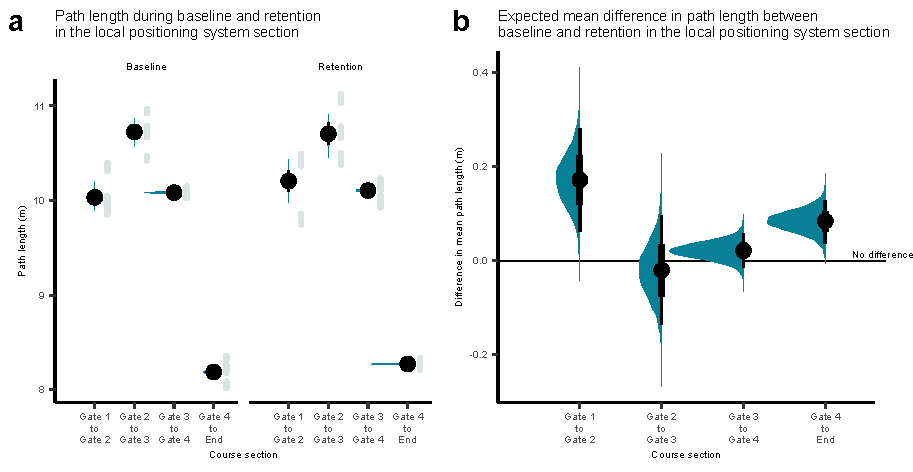
\includegraphics[width=1\linewidth]{figure/figure_path5_2.pdf}
    \caption[Total gate-to-gate path length in the local positioning system section from Study \RNum{1}]{Total gate-to-gate path length in the local positioning system section. \textbf{a.}Estimated gate-to-gate path length during baseline and retention for the local positioning section. \textbf{b.}
Expected mean difference in gate-to-gate path length between baseline and retention in the
local positioning system section. The black lines denote the expected mean or differences in
mean, with the shaded area representing their 95\% credible interval (CI). Each gray point
represents one run trial by a skier.}
    \label{fig:lps_path}
\end{figure}




To conclude, we found that the skiers' speed profiles underwent significant changes, consistent with the changes we would expect from pumping. We also found that the skiers tended to ski a longer path at the retention session, yet accomplished better descent times. However, it is important to consider the limitations of this study, which we discuss further in the methodological section. 

\section{How should we train skiers to ski faster on flat sections in slalom?}


\subsection{Using contextual interference to create challenging problems for skiers did not improve perfor}
Our next question was whether coaches can leverage contextual interference to create learning problems to improve learning. In Study \RNum{1}, the skiers trained to pump on flat sections in slalom either in one course per day (blocked practice) or in different courses randomly assigned each day (interleaved practice). Based on the typical results (at least laboratory-based studies) of the contextual interference effect \cite{simon_metacognition_2001, shea_context_1983, hall_contextual_1994, shea_contextual_1979, tsutsui_contextual_1998, thomas_using_2021}, we hypothesized that the blocked learning group would perform better during the training sessions (acquisition) than the interleaved learning group because they repeatedly skied on the same course and therefore could perfect their performance on this course before switching to the next (thus experiencing less interference). During the first four trials (trial block 1), we found no statistically significant differences between the interleaved and blocked practice groups on course A ($\beta$ = 0.17, 95\% CI[-0.19, 0.53], $t$(91.971) = 0.95, $p$ =  0.344), course B ($\beta$ = -0.03 , 95\% CI[-0.38, 0.33], $t$( 91.241 ) = -0.14, $p$ = 0.886) or course C ($\beta$ = 0.14 , 95\% CI[-0.21, 0.5], $t$(92.069) = 0.81, $p$ = 0.421). Both learning groups improved their race times over the subsequent trial blocks (blocks 2 and 3)(Supplementary Table \ref{paper1: racetimechangepercourse}). However, we found no statistically significant greater improvement in the blocked practice group for any course (Supplementary Table \ref{paper1: racetimeinteraction}). The differences between the learning groups in trial block 2 or trial block 3 were also not statistically significant (Supplementary Table \ref{paper1: racetimedifferencebetweentreatments}). Fig \ref{fig:enter-label})a shows the mean race time estimates for the three trial blocks during acquisition for the three courses. Based on these findings, we did not find evidence that the blocked learning group improved more during the training sessions than the interleaved learning group. 

Our second hypothesis was that the interleaved learning group would outperform the blocked learning group on the retention test conducted after a three-day retention interval. However, we found no evidence against the null hypothesis of no difference between learning groups for course A ($\beta$ = 0.09, 95\% CI[-0.12, 0.3],$t$(45.131) = 0.89 , $p$ = 0.379), B ($\beta$ = 0.13, 95\% CI [-0.18, 0.44], $t$(45.566) = 0.85, $p$ = 0.397), or C ($\beta$ = 0.05, 95\% CI [-0.29, 0.39], $t$(44.813) = 0.29, $p$ = 0.772). To follow up these "null effects", I have fitted the same models as Bayesian models and run a Bayes Factor (BF) analysis to quantify the relative evidence for the two hypotheses to provide additional support for our conclusions. For these analyses, I set the prior for the distribution of differences between the learning groups to 0.05 seconds because values below 0.10 seconds are too small to be considered meaningful. From these models, we found considerable evidence in favor of an absence of an effect of learning group for course A  (BF = 0.972), course B (BF = 0.957), and course C (BF = 0.988). Fig. \ref{fig:ci_bf} shows the prior and posterior distributions for the three slalom courses. Since Bayes Factors are sensitive to model specifications and priors, I performed a sensitivity analysis for different prior distributions but came to the same conclusion. Therefore, we found no convincing evidence that the interleaved learning group improved retention.

\begin{figure}
    \centering
    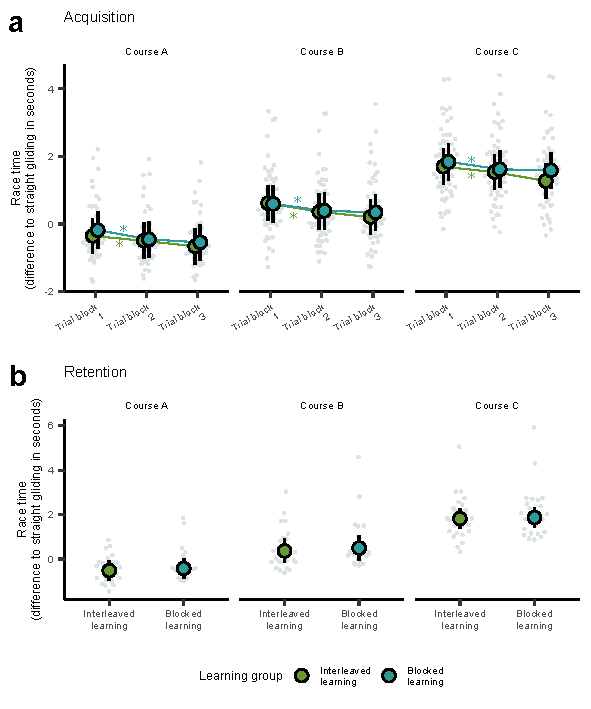
\includegraphics[width=1\linewidth]{figure/figure_results_ci_acquisitionandretention_4.pdf}
    \caption[Race time in the three slalom course across the different sessions for the three learning groups from Study \RNum{1}]{Race time in the three slalom course across the different sessions for the three learning groups. \textbf{a}. Estimated race times during the three acquisition trial blocks (1, 2, 3). \textbf{b.} Estimated race times for retention. Intervals represent the 95\% confidence intervals (CIs) derived from the models. Each light gray point represents a single trial performed by a skier. The figure is based on the data and results from \cite{magelssen_is_2022}.}
    \label{fig:ci_results}
\end{figure}

\begin{figure}
    \centering
    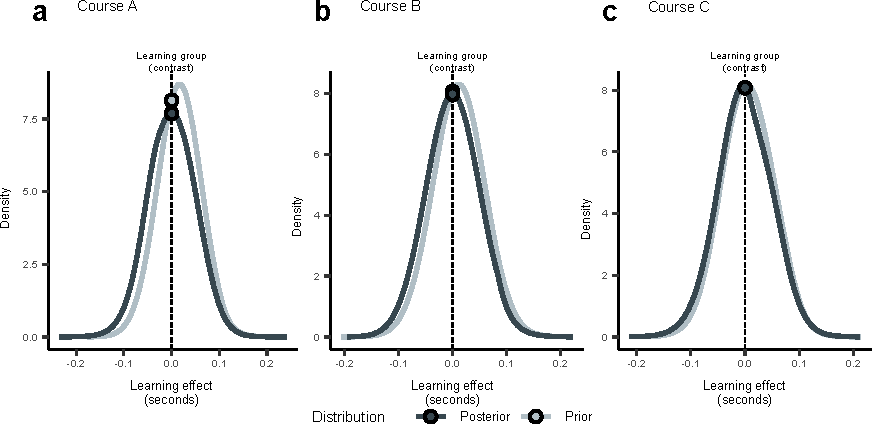
\includegraphics[width=1\linewidth]{figure/figure_results_BF_4.pdf}
    \caption[The relative evidence for the two hypotheses in the three slalom courses]{The relatiWve evidence for the two hypotheses in the three slalom courses using Bayes Factors for comparison. The ratio represents Savage-Dickey ratio.}
    \label{fig:ci_bf}
\end{figure}

To begin, our study aligns with previous research that has not found a contextual interference effect in real-world tasks or more complex activities \cite{brady_theoretical_1998, barreiros_contextual_2007, wulf_principles_2002}. One reason for this is that the skiers were skilled, and the sport is complex. A comparable study revealed no significant effect of frequent task switching (alternating between two types of serves in the interleaved learning group) on learning tennis serves among younger players\cite{buszard_quantifying_2017}. However, the tennis players in this interleaved learning groupW improved their serves in competition (transfer) compared to those in the blocked learning group. In contrast, \cite{hall_contextual_1994} found that baseball players batted better after training with interleaved learning over several weeks than after training with blocked learning. The key difference between these two studies is that the former manipulated contextual interference between two different skill types, while the latter manipulated variations of the same skill. Therefore, the way the manipulation was performed (between skills versus between variations of one skill) might be a contributing factor. However, our study is most consistent with the manipulation type in \cite{hall_contextual_1994} study and should have corroborated the findings from that study. Therefore, it appears that this is not the best explanation for our data.

Another reason for the difference in results between our study and previous studies on contextual interference is that skiing is a continuous skill, while most of the literature focuses on learning discrete skills\cite{lee_distribution_1988, lee_distribution_1989}. Although contextual interference has been found for continuous tasks\cite{pauwels_contextual_2014, tsutsui_contextual_1998}, these findings come from beginners and relatively simple tasks. According to the 3R framework of motor learning \cite{tsay_strategy_2023}, skilled performers are adept at recognizing changes in the learning environment and quickly adapt their control policy to improve performance if a better alternative exists. Therefore, the skiers in the interleaved learning group may not have experienced significant interference because they quickly identified the new task and quickly switched to a more effective control policy. Since ski runs endure over a long time, skiers could adjust their control policy within the first few gates without significantly compromising their performance.

A third potential counteracting factor of the contextual interference effect in our study was the long rotation time between each run, which may have contributed to forgetting. Skiers took approximately 8 minutes between trials to ride the lift to the top and prepare for a new run. This intertrial interval is significantly longer than those used in laboratory tasks with discrete tasks \cite{barreiros_contextual_2007}. The extended time between trials might have caused skiers to forget and lose connections between trials, which is a mechanism suggested to underlie the contextual interference effect \cite{lee_locus_1983, lee_can_1985}. This perspective also aligns with the new theory of disuse \cite{bjork_new_1992}, which posits that lengthening the spacing between trials can increase forgetting yet enhance learning by reducing memory retrieval strength before each trial. Thus, both the interleaved and blocked groups might have experienced favorable learning conditions for skill learning due to the long intertrial.

Although we did not find significant differences between the learning groups, this does not imply that we do not recommend coaches frequently switch courses to create learning problems for skiers. Our findings only suggest that within the short duration of our training study (equivalent to a typical ski camp), we found no convincing benefits of interleaved learning. However, an important general training principle is the specificity principle \cite{lee_chapter_1988}, which states that training should meet the demands of the sport. In alpine skiing, skiers constantly encounter new competition courses, making it crucial for training to cover this range of variation. Frequently changing courses could help avoid the formation of undesirable habits \cite{du_relationship_2022}, such as skiers learning a solution to a situation only by perfecting it on a single course. While our study did not provide data to support this, it is a potential area for future research.

One limitation of this study is that the interleaved and blocked learning groups trained together, which could have created some treatment diffusion when the skiers observed each other from the lift or the top of the course. Unfortunately, we were unable to control for this potential limitation in this study due to space and time constraints in the ski hall. Another limitation is the absence of a transfer test, which could have provided important insights into the learning groups’ adaptation to a new slalom course.

To conclude, we did not find convincing evidence that coaches could leverage contextual interference to design challenging learning problems to improve learning.

\subsection{Using reinforcement-guided teaching signals improved training and performance compared to supervised-guided teaching signal}
The final question this doctoral study addressed was which teaching signal is most effective for teaching skiers to make optimal strategy choices, thereby impacting their performance and learning. In Study \RNum{2}, skiers learned the value of different strategies through two opposing teaching signals: supervised learning and reinforcement learning. In the supervised (free choice) learning group, coaches instructed skiers on which strategy to use, either one they believed to be the best or most appropriate for the skier. This method represents the conventional teaching strategy in alpine skiing. To complement this learning group, we included a supervised (target skill) learning group, which served as a benchmark for the upper limit of performance achievable through optimal strategy choices. In this learning group, coaches instructed skiers to select the strategy we defined as theoretically best based on mechanics and field observations of elite skiers. We compared these two supervised learning groups to a reinforcement learning group, where skiers learned the values of the strategies by trying them and learning from evaluations (that is, race times) instead of from a coach. 






\begin{figure}
    \centering
    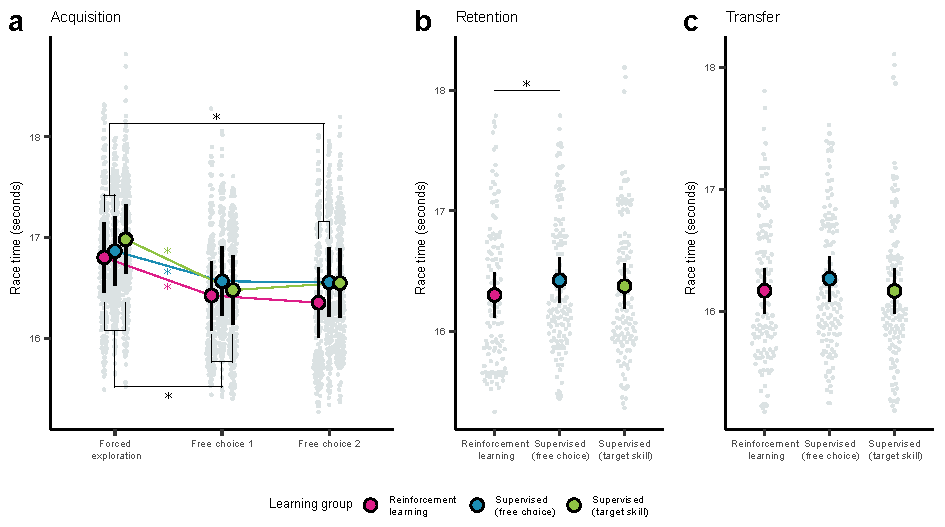
\includegraphics[width=1\linewidth]{figure/figure_racingtimes_2.pdf}
    \caption{Race time across the different sessions for the three learning groups \textbf{a}. Estimated race times during the three acquisition sessions. Forced exploration refers to the sessions wherein skiers tried all strategies, whereas free choice 1 and free choice 2 refer to the session wherein skiers or coaches selected strategies according to their assigned learning groups. \textbf{b.} Estimated race times for retention. \textbf{c.} Estimated race times for transfer. Intervals represent the 95\% confidence intervals (CIs) derived from the models. Asterisks (*) indicate a statistically significant effect. Each light gray point represents a single trial performed by a skier.}
    \label{fig:rlstudy_racetime}
\end{figure}

Tp begin, we expected the reinforcement learning group to improve their race time more during the three acquisition sessions than did the supervised (free choice) learning group. We hypothesized that this improvement would come about from improved learning to select effective strategies. Importantly, we did not expect the reinforcement learning group to select better strategies than the supervised (target skill) learning group because this group was instructed to select the theoretical best strategy. First, we analyzed the differences between the learning groups during the forced exploration acquisition session, where all groups were required to try all strategies. Therefore, we did not expect to find differences between the groups at this session. The results confirmed our expectations; we found no statistically significant differences between the reinforcement learning group and the supervised (free choice) learning group ($\beta$ = 0.06, 95\% CI [-0.2, 0.32], $t$(92.727) = 0.48, $p$ = 0.631) or between the supervised (target skill) learning group  ($\beta$ = 0.18, 95\% CI[-0.08, 0.44], $t$(92.663) = 1.37, $p$ = 0.174).  

When we allowed the learning groups to choose their own strategies—skiers in the reinforcement learning group and coaches in the two supervised learning groups—during the next two sessions in acquisition (free choice sessions 1 and 2), we expected them to show the development patterns described above. First, we observed that all learning groups significantly improved their race times over the course of the free -choice sessions during acquisition (Supplementary Table \ref{table_racetime_acquisition_change}). The improvements across these sessions indicate that the choice of strategies exerted a great influence on race time in all the learning groups. Consistent with our expectations, the three learning groups also developed differently. The supervised (target skill) learning group, where skiers were coached to select the theoretically best strategy, showed a significantly greater improvement than the reinforcement learning group from forced exploration to free choice 1 ($\beta$ = -0.12, 95\% CI[-0.22, -0.03], $t$(91.777) = -2.58, $p$ = 0.012). Conversely, the supervised (free choice) learning group demonstrated a descriptively poorer progression than the reinforcement learning group, although this difference was not statistically significant ($\beta$ = 0.08, 95\% CI[-0.02, 0.17], $t$(92.5) = 1.61, $p$ = 0.110). Continuing this trend, comparing initial performance during forced exploration to performance in the final acquisition session (free choice 2), the reinforcement learning group improved significantly more than did the supervised (free choice) learning group ($\beta$ = 0.14, 95\% CI[0.02, 0.26], $t$(95.743) = 2.26, $p$ = 0.026). For the same comparison, the supervised (target skill) learning group no longer showed significantly greater improvement than the reinforcement learning group  ($\beta$ = 0.02, 95\% CI[-0.11, 0.14], $t$(95.651) = 0.26, $p$ = 0.798). This is due in part to the continued improvement of the reinforcement learning group but also to a descriptive decline from free choice 1 to free choice 2 in the supervised (target skill) learning group, attenuating their initially greater improvement rate. However, we did not find statistical evidence that the reinforcement learning group performed better than the supervised (free choice) or supervised (target skill) learning groups at free choice 1 or free choice 2 (Supplementary Table \ref{table_racetime_acquisition_groupdifference}). Fig. \ref{fig: racetime}a presents the mean race time estimates during the three acquisition sessions. 

In the retention session, the skiers independently chose their strategies, irrespective of their assigned groups. We reasoned that at this point, the reinforcement learning group had learned to understand which strategies were most effective and chose them. Therefore, our hypothesis was that the reinforcement learning group would outperform the supervised (free choice) learning group in retention due to better strategy selection learned from observing the race times to evaluate the strategies. Consistent with this hypothesis, we found that the reinforcement learning group performed significantly better than the supervised (free choice) learning group did ($\beta$ = 0.12, 95\% CI[0.01, 0.24], $t$(101.422) = 2.12, $p$ = 0.037). The difference between the reinforcement learning and supervised (target skill) learning groups also favored reinforcement learning but was smaller and not statistically significant  ($\beta$ = 0.07, 95\% CI[ -0.04, 0.19], $t$(101.63) = 1.27, $p$ = 0.206). We therefore provide evidence that the reinforcement learning group performed better at retention than did the supervised (free choice) learning group. Descriptively, the reinforcement learning group performed better, even than the supervised (target skill) learning group, which served as an upper bound reference. Fig. \ref{fig: racetime}b presents the mean race time estimates during retention. 

We also hypothesized that reinforcement learning would transfer their skill learning to a new slalom course compared to the supervised (free choice) learning group. Similar to retention, the reinforcement learning group performed better than the supervised (free choice) group but the difference was smaller and not statistically significant ($\beta$ = 0.1, 95\% CI[-0.02, 0.21], $t$( 99.979) = 1.7, $p$  = 0.091). The race times for the reinforcement learning and supervised (target skill) learning groups were on average identical ($\beta$ = 0, 95\% CI[-0.12, 0.11], $t$(100.033) = -0.04, $p$ = 0.967). Therefore, we did not find convincing evidence that reinforcement learning improved transfer. Fig. \ref{fig: racetime}c presents the mean race time estimates during the transfer session. 

We proposed that the enhanced performance of the reinforcement learning group, compared to the supervised (free choice) group, came about from better strategy selection because they learned the strategies' values directly from observing their race times. We tested this prediction by examining whether the reinforcement learning group developed a greater probability of choosing the theoretically best strategy ("extend with rock skis forward") or each skier's estimated best strategy over the free choice sessions in the acquisition and retention and transfer sessions. However, no convincing evidence was found for this hypothesis with any of these tests. Instead we found support for two other explanations. First, we found that the skiers in the reinforcement learning group who made 'suboptimal' choices during the retention session had a lower 'cost'—the expected difference between a suboptimally chosen strategy and the skier's estimated best strategy—than the skiers in the supervised (free choice) learning group. The reinforcement learning group, therefore, appears to have learned to select strategies that offered comparable outcomes and to avoid those that carried the risk of substantially worse performance. Second, we found that the reinforcement learning group improved more on the 'extend' strategy over the course of the sessions than did the supervised (free choice) learning group. One possibility is that the reinforcement learning group discovered that the "extend" strategy alone provided almost the full benefits on its own and chose this strategy because it was simpler than "extend with rock skis forward", subsequently refining this strategy. I have chosen not to include figures or results in this thesis due to space constraints. For complete results and discussion, see paper \RNum{3}.

Our results suggest that reinforcement learning can prove to be a useful teaching strategy for improving training and performance among elite athletes. The estimated group difference was substantial and may have exerted a real impact on skiers' skill development. Assuming that a full slalom course of approximately 45 seconds includes a flat section lasting approximately 15 seconds (quite typical), and considering that a slalom race consists of two runs, the 0.12-second difference can translate into an improved Fédération Internationale de Ski (FIS) world ranking of 27 positions for females and 65 positions for males, based on a median ranking of 600 in our sample (see Supplement Discussion \textbackslash{}ref\{supdiscussion\}). However, it is important to note that the estimated effect is still smaller than our smallest effect size of interest, a benchmark set for other conditions that we were unable to fulfill due to time and space limitations in the ski hall. 

One limitation of the study is that we did not use motion capture to analyze the skiers' execution of the strategies. Consequently, we cannot describe the actual execution of the strategies beyond noting that they were able to perform them during the familiarization test. Based on our results, it is likely that the reinforcement learning group learned not only at the strategy level but also at an execution level, which we were unable to quantify in this study.






 

\chapter{General discussion}
In recent decades, cognitive science has deepened our understanding of the mechanisms that subserve skill learning and has begun to spark ideas on how to achieve better learning by leveraging these mechanisms more effectively. Thus far, most studies have focused on simple, laboratory-based tasks, raising concerns about their applicability to real-world learning in areas such as sports, education, or rehabilitation. Therefore, there is a pressing need for studies with greater ecological validity, where learning tasks are not trivial exercises but instead improve important life functions or skills that learners genuinely care about. The overarching goal of this doctoral thesis was to bridge this gap between simple tasks and real-world skill learning with skilled performers using alpine skiing as a domain to test these theories. To achieve this goal, this doctoral thesis adopted a crossdisciplinary research approach involving mechanics and psychology. From a mechanical perspective, we asked what is the most effective strategies for skiing faster on flat slopes (aim 1) and the kinematic signatures that make one of these strategies so effective (aim 2). From a psychological perspective, we asked whether better learning effects could be achieved by applying learning theories from cognitive science to create learning problems (aim 3) and better utilize teaching signals (aim 4).  

First, we found that skiers on average achieved the fastest race times using the "extend with rock skis forward" strategy, which aligns with our expectations based on theory and quantitative field observations. This suggests that this strategy is powerful and can improve the performance of skiers on flats in slalom. However, its effect was only marginally better than that of the "extend" strategy, which is simpler and nearly as effective on its own. Based on these results, we recommend that skiers choose either of these two strategies to enhance their performance on flat sections in slalom. These findings expand upon previous ski research and provide experimental evidence for effective strategies to ski fast on flats in slalom.

Second, we also found that a training intervention focusing on the "extend" strategy left a remarkable kinematic signature on the skiers. After the intervention, skiers exhibited a more wave-like speed profile. That is, they increased their speed after passing through a gate, which continued to rise until they were approximately midway between two gates. Then, their speed decreased until the next gate, before increasing again. Additionally, we observed a trend where skiers took longer paths between gates, yet their race times improved. Together, these kinematic signatures closely resemble the predictions from Lind and Sander's model of pumping to increase velocity. A limitation of our data is that we do not know the specific movements the skiers made, preventing us from testing the model's predictions accurately. Future research should employ motion capture technology to achieve the necessary data quality for such investigations.

Shifting focus toward the testing of learning theories to improve skill learning, we did not find evidence that the skiers learned better by increasing the frequency at which they were exposed to new learning problems (that is, interleaved practice). This finding aligns with prior research that has similarly failed to observe a contextual interference effect in real-world tasks or more complex learning tasks \cite{brady_theoretical_1998, barreiros_contextual_2007, wulf_principles_2002}. Based on the results of this study and these previous findings, it may not be worthwhile to expend effort in creating multiple different slalom courses, at least concerning performance outcomes. Nonetheless, we should not dismiss the possibility that exposing skiers to rapid changes in course could influence other cognitive mechanisms. It is also plausible that the benefit of frequent course changes lies in preventing habits \cite{du_relationship_2022}, whereby skiers settle on a fixed solution and become insensitive to adapting to different situations. If so, simply changing courses sufficiently often might be adequate to avoid these habits. To better understand this phenomenon, an alternative experimental design is crucial. One approach could involve training hairpin, with one learning group practising only one hairpin while another group practising multiple hairpins.

Til slutt fant vi at å lære strategier og deres verdier gjennom med reinforcement learning var et mer effektive teaching signal enn convential instruction-based teaching with a coach.  Interestingly, the reinforcement learning group also performed descriptively better than the supervised (target skill) learning group, which was meant to serve as a benchmark for the upper limit of performance achievable through optimal strategy choices. I tillegg var effektstørrelsen av såpass størrelse at den potensielt kan ha exerted real impact on skiers world ranking based on their FIS points. Våre prediksjoner om at denne gruppeforskjellen was caused by better strategy selection on the single best strategy did not prove succesful. That is, the reinforcement learning group did not begin with or develop a greater probability of choosing the theoretically optimal strategy or the individual skier's estimated best strategy compared with the supervised (free choice) learning group. Instead, we found that the expected loss in time for skiers who made 'suboptimal' choices (that is, cost or expected regret) during the retention var lavere i reinforcement learning group than did the skiers in the supervised (free choice) learning group. One way to interpret this is that the reinforcement learning group appears to have learned to select strategies that offered comparable outcomes and to avoid those that carried the risk of substantially worse performance. One possibility is that the reinforcement learning group discovered that the "extend" strategy alone almost provided full benefits on its own and chose this strategy because it was simpler than "extend with rock skis forward". See Paper \RNum{3} for complete results and discussion.

The findings from this study suggest that reinforcement learning can serve as an effective teaching signal for selecting optimal strategies and performance. The key question is how coaches or teachers can apply this knowledge in practice. One approach is to replicate the strategies developed in the study and teach skiers to use them. However, the application can be simplified or made more advanced depending on the skill level or experience of the skiers. For less skilled skiers, learning can occur by having them ski high and low in hockey to observe the impact on their times, or by creating multiple line choices around a gate and allowing skiers to experiment with them. For more skilled skiers, a narrower set of strategies that are expected to produce smaller yet meaningful and interpretable differences can be developed. The general principle to make reinforcement learning effective is to design strategies that challenge expectations, ideally with one strategy outperforming the expected outcomes. Once skiers have established a solid understanding of the value of different strategies, it may become less useful to continue gaining experience with those strategies. At this point, coaches can either develop new sets of strategies or shift their learning strategy, such as focusing on refining the execution of the strategies. 




Avslutningsvis har jeg lyst til å evaluere den interdisiplinære tilnærmingen mellom mekanikk og psykologi for å studere skill learning in skilled athletes. 


First, some of the strategies we created based on mechanics and quantative observations of elite skiers in the field proved effective in improving skiers' race times, with some skiers improving by more than two seconds from an already high skill level. For many athletes, these strategies provided an "aha" moment. And when they realizing the power of these strateiges, they began pushing themselves further and further improved their performances. Our observations align with previous studies, which have shown that developing new strategies is crucial for continued progress. As word spread within the skiing community that our research was not just academic but genuinely improved skiers' performances, we experienced an increased interest for participating in the study. In total, we tested 186 skilled alpine skiers from Norway and Sweden, including those who served as pilot participants. All these ski teams covered their own travel and accommodation costs themselves, demonstrating the commitment and interest from the sports community. 

Fra et idrettsfaglig perspektiv er resultatene fra strategiene interessante i seg selv. Men det aller mest interessante resultatet kommer ved å trekke inn psykologi for å teste hvilket teaching signal som er mest effektive for å lære disse strategiene. Det er dette treffpunktet som har vært det unike med doktorgraden, der man lære hvilke strategier som er effektive og samtidige undersøke hvilke læringsstrategier som er mest effektive for å lære disse. Det gjør at læringseksperimentene blir så virkelighetsnært som mulig, og øker sannsynligheten for at utøvere lærer gjennom intervensjonen og at de prioriterer å bli med i prosjektet.

En utfordring med den tverrfaglige tilnærmingen er at den krever god kunnskap om både idrettens egenart og mekanikk og psykologi. Norges idrettshøgskole har vært verdenskjent for sitt gode vitenskapelige miljø på alpint der studenter har blitt godt skolert i idrettens egenart og forståelse av svingteknikk. Det er blant annet denne forståelsen av svingteknikk som vi har tuftet strategiene på. Samtidig krever den solid kunnskap om psykologi, slik at man ser disse koblingene mellom hva idretten trenger og hvilke spørsmål som psykologifaget er interessert i. Det er mange som har god kompetanse om 













Først av alt var strategiene vi lagde med forankring i mekanikk effektive for å forbedre utøveres skikjøring, og enkelte utøvere forbedret seg med over to sekunder fra et allerede høyt ferdighetsnivå. For mange utøvere ga strategiene en slags aha opplevelse. Og da det gikk opp for dem at de kunne gjøre ting annerledes og at det var mer effektive strategier enn de allerede var kjent med, prøvde de mer og forbedret sine prestasjoner ytterligere. Vår observasjon viser slående likheter med tidligere studier der man finner at utvikling av nye strategier er avgjørende for å sikre videre fremgang. Da det ble kjent i skimiljøet at utøvere ikke bare ble forsket på for forskningen sin skyld, men at strategiene faktisk forbedret utøverne sine prestasjoner var ønsket om å delta i studien stort. Totalt har vi testet 186 gode alpinister fra Norge og Sverige, inkludert skikjørere som deltok som piloter. Alle disse lagene dekket alle reise og overnattingskostnader selv, hvilket viser engasjementet og interessen fra idrettens sin side. 

Selv om man kunne gjort læringsintervensjoner på disse strategiene i seg selv er det mer 








et godt stimuli for læring.  Sikret at mange ble i prosjektet.  



tilnærmingen helt avgjørende for å oppnå fremgang hos utøvere. I begge studiene var fremgangen til utøverne i gjennomsnitt substantial, og enkelte utøvere forbedret seg med over to sekunder fra et allerede høyt nivå på den korte sekvensen. For mange ga strategiene vært en -aha opplevelse, og et godt stimuli for læring.  Sikret at mange ble i prosjektet. 




En hjørnestein for prosjektet var også den interdisiplinære tilnærmingen mellom mekanikk og psykologi, som har vært helt avgjørende for å få til fremgang hos utøvere. I begge studiene har fremgangen til utøverne vært enorm, og enkelte utøvere har forbedret seg med over to sekunder fra et allerede høyt nivå på den korte sekvensen. For mange har strategiene vært en -aha opplevelse, og et godt stimuli for læring. 




\section{Methodological considerations}



\subsection{Quantifying performance in alpine skiing}
One of the key objectives of this doctoral project was to determine a reliable method for quantifying performance in alpine skiing over time, whether over days, weeks, or months. One of the greatest challenges in this respect, from a scientific perspective, is its lack of standardization; the time taken to ski a slalom course one day may not be comparable to that of another day  Consequently, quantifying performance in alpine skiing has been widely debated, with scientists arguing for measures such as energy mechanics \cite{supej_differential_2008, supej_how_2010, supej_mechanical_2011} , differences in mechanical energy divided by time, section times \cite{supej_relations_2006}, lateral skidding of skis \cite{kirby_development_2009}, and time loss per elevation difference and distance travelled per elevation difference \cite{federolf_quantifying_2012}. Throughout my doctoral research, I have chosen to express performance in terms of time, which is the conventional way to quantify performance in skiing and allowed me to operate on the same scale as skiers and coaches do. In my doctoral reseach, I have adopted two different time measures: in papers 1 and 2, I have expressed time as the difference from the time when the skier skied the section straight down (straight gliding), whereas, in paper 3, I used the raw time to quantify performance. Here, I aim to provide some methodological reflections on these approaches to help readers evaluate the results of the studies in this doctoral thesis and to assist other researchers in the field of alpine skiing. 

To begin this methodological consideration, I conducted a Bayesian multilevel growth model on all the skiers' times as they skied straight down the section for all sessions in paper 3. From this analysis, I found that the straight gliding times for all ski groups (A, B, C, and D) increased steadily from the first session (baseline) to the last session (transfer). Although I cannot rule out any explanation for why the straight gliding times of the ski groups increased uniformly, I am confident that differences in the length of the course section are not the main explanation. This is because we used a measuring tape during the course setting, and there was a tight cluster of boreholes at the finish line, with only a few centimeters of difference. I also do not believe that changes in the skiers' starting procedures or execution of straight gliding are the main reasons. This is because the skiers were diligent and interested in performing this task as well as possible. I believe the best explanation involves the snow conditions and how we prepared them. Specifically, when grooming snow with a machine, grooves are left in the snow that becomes hard if it is watered and allowed to freeze. These hard grooves are fast to ski on because only a small part of the ski is in contact with the snow surface. As skiers complete more runs and coaches slide through the course, these snow grooves wear away, creating a smooth, hard base without grooves. When skiers descend on this groom-free base, a larger part of the ski’s contact surface touches the snow, which increases ski–snow friction and slows the skiers down.

The question is, what consequences does this have for the results, and how can we address these challenges the best possible way? First, one challenge this creates is the need to exercise caution in interpreting 'true' learning from the estimated change in race times. From From Fig. \ref{fig:rlstudy_racetime} from Study \RNum{2}, we find that the skiers improved their race times significantly over the sessions despite the increased straight gliding times. Therefore, the 'true' improvement is likely better than estimated. A less conservative and perhaps better way to express skiers' 'true' learning is to use the difference in straight gliding times for each session to account for variations in the snow surface. This is the performance measure we used in Study\RNum{1}. However, although this measure may better capture skiers' learning, we do not know whether it underestimates or overestimates learning. Another problem is that straight gliding in itself is a random variable that introduces variation and could add noise to the measurement. In Study \RNum{2}, we had to move away from this measure because the straight gliding lane crossed many holes from the previous courses. Due to these challenges, it is difficult to determine the actual improvement of skiers. Scientists therefore face two choices: either use raw race times, which is likely a conservative method that underestimates the real improvement, or express time as the difference in straight gliding, which may better account for variations in the surface and therefore express progress more accurately. The cost of the latter approach is that it underestimates or overestimates performance and could increase noise. 

Another solution is to downplay the focus on change and determine whether the learning groups differ on the postmeasure if their performance is equal at baseline, corresponding to the logic of an ANCOVA. If we have a design where skiers have undeone tests simultaneously, we can estimate this group difference, indirectly avoiding the question of change. Therefore, we used ANCOVA and raw race data in Study \RNum{2}.

One potential way to improve estimates in future research is to test more levels within the ski groups. This would allow the groups to have varying effects of the treatment and achieve better estimates through partial pooling \cite{mcelreath_statistical_2018}. We attempted to run this model, but it did not converge due to having too few levels. It might have been better to divide the ski groups into smaller subgroups that were tested at different times. This approach could have provided more levels and potentially better estimates through partial pooling. However, it must be emphasized that conducting studies such as ours is very difficult and time-consuming. Another approach is to skid extensively to eliminate the grooms before testing. 


\begin{figure}
    \centering
    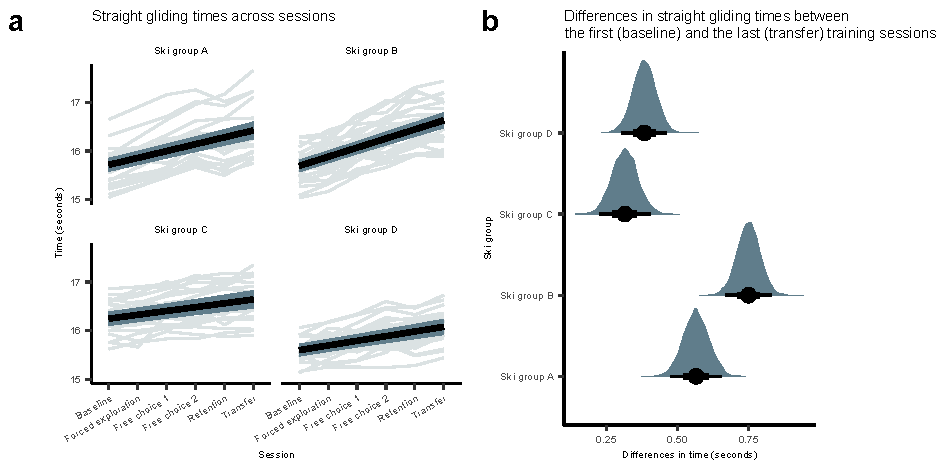
\includegraphics[width=1\linewidth]{figure/figure_methodological_straightgliding.pdf}
    \caption{Enter Caption}
    \label{fig:straightgliding}
\end{figure}

\chapter{Appendix Thesis}


\section*{Details of statistical models}\label{study3:estimateddifferencebetweenstrategies}

Model 1: Differences in race times between the strategies during the forced exploration session

\begin{verbatim}
brm(formula = racingtime ~ 0 + strategy + 
          (0 + strategy | skier),
    prior = c(prior(normal(16, 0.5), class = b),
              prior(exponential(1), class = sigma),
              prior(exponential(1), class = sd)),
    control = list(adapt_delta = 0.95),
    family = gaussian)
\end{verbatim}

\clearpage

\section*{Supplementary tables for Study \RNum{1}}\label{study1:CIracetime}

\afterpage{
\begin{table}[ht]\label{paper1: racetimedifferencebetweentreatments}
\centering
\begin{threeparttable}
\caption{Race times: difference between the learning groups for each course at each trial block}\label{paper1: racetimedifferencebetweentreatments}
\begin{tabular}{llrrrrrrl}
  \hline
Term & Estimate & SE & df & CI & t & p \\ 
  \hline
(Intercept) & 0.52 & 0.21 & 5.81 & -0.01-1.05 & 2.44 &    0.052 \\ 
block 2 & -0.21 & 0.03 & 499.93 & -0.28--0.14 & -6.29 &  $<$  0.001 \\ 
block 3 & -0.33 & 0.03 & 500.58 & -0.40--0.27 & -9.72 &  $<$  0.001 \\ 
course B & 0.87 & 0.03 & 499.63 & 0.80-0.93 & 25.70 &  $<$  0.001 \\ 
course C & 2.04 & 0.03 & 503.12 & 1.97-2.11 & 59.69 &  $<$  0.001 \\ 
block 2 : course B & -0.02 & 0.08 & 499.43 & -0.18-0.14 & -0.25 &    0.801 \\ 
block 3 : course B & 0.01 & 0.08 & 499.47 & -0.16-0.17 & 0.07 &    0.940 \\ 
block 2 : course C & 0.02 & 0.08 & 499.43 & -0.14-0.18 & 0.25 &    0.804 \\ 
block 3 : course C & -0.00 & 0.08 & 499.45 & -0.17-0.16 & -0.02 &    0.988 \\ 
block 1 : course A : blocked & 0.17 & 0.18 & 91.97 & -0.19-0.53 & 0.95 &    0.344 \\ 
block 2 : course A : blocked & 0.04 & 0.18 & 92.64 & -0.32-0.40 & 0.23 &    0.818 \\ 
block 3 : course A : blocked & 0.12 & 0.18 & 96.10 & -0.24-0.48 & 0.66 &    0.509 \\ 
block 1 : course B : blocked & -0.03 & 0.18 & 91.24 & -0.38-0.33 & -0.14 &    0.886 \\ 
block 2 : course B : blocked & 0.03 & 0.18 & 91.91 & -0.32-0.39 & 0.18 &    0.859 \\ 
block 3 : course B : blocked & 0.14 & 0.18 & 95.30 & -0.22-0.50 & 0.77 &    0.444 \\ 
block 1 : course C : blocked & 0.14 & 0.18 & 92.07 & -0.21-0.50 & 0.81 &    0.421 \\ 
block 2 : course C : blocked & 0.08 & 0.18 & 92.74 & -0.27-0.44 & 0.46 &    0.646 \\ 
block 3 : course C : blocked & 0.31 & 0.18 & 97.04 & -0.05-0.68 & 1.73 &    0.088 \\ 
sd(Intercept) & 0.64 &  &  &  &  &   \\ 
sd(Intercept) & 0.46 &  &  &  &  &   \\ 
sd(Observation) & 0.33 &  &  &  &  &   \\ 
   \hline
\end{tabular}
\begin{tablenotes}
\item[1] Formula: racetime $\sim$ trialblock * course / treatment + (1 $|$ skier) + (1 $|$  skiacademy)
\end{tablenotes}
\end{threeparttable}
\end{table}


\begin{table}[ht]
\centering
\begin{threeparttable}
\caption{Race times: change per course for each treatment}\label{paper1: racetimechangepercourse}
\begin{tabular}{llrrrrrrl}
  \hline
Term & Estimate & SE & df & CI & t & p \\ 
  \hline
(Intercept) & 0.52 & 0.21 & 5.81 & -0.01-1.05 & 2.44 &    0.052 \\ 
course B & 0.87 & 0.03 & 499.63 & 0.80-0.93 & 25.70 &  $<$  0.001 \\ 
blocked & 0.11 & 0.16 & 61.90 & -0.21-0.44 & 0.70 &    0.488 \\ 
course B : blocked & -0.06 & 0.07 & 499.63 & -0.20-0.07 & -0.92 &    0.357 \\ 
course A : interleaved : block 2 & -0.15 & 0.08 & 499.79 & -0.30-0.01 & -1.84 &    0.066 \\ 
course B : interleaved : block 2 & -0.26 & 0.08 & 499.79 & -0.41--0.10 & -3.28 &    0.001 \\ 
course C : interleaved : block 2 & -0.16 & 0.08 & 499.79 & -0.31--0.00 & -2.01 &    0.045 \\ 
course A : blocked : block 2 & -0.27 & 0.08 & 499.43 & -0.44--0.11 & -3.25 &    0.001 \\ 
course B : blocked : block 2 & -0.20 & 0.08 & 499.43 & -0.37--0.04 & -2.43 &    0.016 \\ 
course C : blocked : block 2 & -0.22 & 0.08 & 499.43 & -0.39--0.05 & -2.61 &    0.009 \\ 
course A : interleaved : block 3 & -0.31 & 0.08 & 500.19 & -0.47--0.15 & -3.79 &  $<$  0.001 \\ 
course B : interleaved : block 3 & -0.41 & 0.08 & 500.19 & -0.57--0.25 & -5.02 &  $<$  0.001 \\ 
course C : interleaved : block 3 & -0.42 & 0.08 & 500.19 & -0.58--0.26 & -5.14 &  $<$  0.001 \\ 
course A : blocked : block 3 & -0.36 & 0.09 & 499.52 & -0.53--0.19 & -4.23 &  $<$  0.001 \\ 
course B : blocked : block 3 & -0.25 & 0.08 & 499.50 & -0.41--0.08 & -2.95 &    0.003 \\ 
course C : blocked : block 3 & -0.25 & 0.09 & 499.58 & -0.42--0.08 & -2.93 &    0.004 \\ 
sd(Intercept) & 0.64 &  &  &  &  &  \\ 
sd(Intercept) & 0.46 &  &  &  &  &   \\ 
sd(Observation) & 0.33 &  &  &  &  &  \\ 
   \hline
\end{tabular}
\begin{tablenotes}
\item[1] Formula: racetime $\sim$ course * treatment / trialblock + (1 $|$ skier) + (1 $|$ skiacademy)
\end{tablenotes}
\end{threeparttable}
\end{table}


\begin{table}[ht]
\caption{Race times: differences in improvement across trial blocks}\label{paper1: racetimeinteraction}
\centering
\begin{threeparttable}
\begin{tabular}{llrrrrrrl}
  \hline
Term & Estimate & SE & df & CI & t & p \\ 
  \hline
(Intercept) & 0.52 & 0.21 & 5.81 & -0.01-1.05 & 2.44 &    0.052 \\ 
course B & 0.87 & 0.03 & 499.63 & 0.80-0.93 & 25.70 &  $<$  0.001 \\ 
course C & 2.04 & 0.03 & 503.12 & 1.97-2.11 & 59.69 &  $<$  0.001 \\ 
block 2 & -0.21 & 0.03 & 499.93 & -0.28--0.14 & -6.29 &  $<$  0.001 \\ 
block 3 & -0.33 & 0.03 & 500.58 & -0.40--0.27 & -9.72 &  $<$  0.001 \\ 
course A : blocked & 0.11 & 0.17 & 69.34 & -0.22-0.44 & 0.66 &    0.509 \\ 
course B : blocked & 0.05 & 0.17 & 69.06 & -0.28-0.38 & 0.29 &    0.772 \\ 
course C : blocked & 0.18 & 0.17 & 69.52 & -0.15-0.51 & 1.08 &    0.283 \\ 
course B : block 2 & -0.02 & 0.08 & 499.43 & -0.18-0.14 & -0.25 &    0.801 \\ 
course C : block 2 & 0.02 & 0.08 & 499.43 & -0.14-0.18 & 0.25 &    0.804 \\ 
course B : block 3 & 0.01 & 0.08 & 499.47 & -0.16-0.17 & 0.07 &    0.940 \\ 
course C : block 3 & -0.00 & 0.08 & 499.45 & -0.17-0.16 & -0.02 &    0.988 \\ 
course A : blocked : block 2 & -0.13 & 0.12 & 499.60 & -0.36-0.10 & -1.11 &    0.265 \\ 
course B : blocked : block 2 & 0.06 & 0.11 & 499.60 & -0.17-0.28 & 0.50 &    0.615 \\ 
course C : blocked : block 2 & -0.06 & 0.12 & 499.60 & -0.29-0.17 & -0.54 &    0.591 \\ 
course A : blocked : block 3 & -0.05 & 0.12 & 499.85 & -0.28-0.18 & -0.43 &    0.671 \\ 
course B : blocked : block 3 & 0.16 & 0.12 & 499.83 & -0.07-0.40 & 1.41 &    0.160 \\ 
course C : blocked : block 3 & 0.17 & 0.12 & 499.88 & -0.06-0.40 & 1.42 &    0.156 \\ 
sd(Intercept) & 0.64 &  &  &  &  &   \\ 
sd(Intercept) & 0.46 &  &  &  &  &    \\ 
sd(Observation) & 0.33 &  &  &  &  &    \\ 
   \hline
\end{tabular}
\begin{tablenotes}
\item[1] Formula: racetime $\sim$ course / treatment * trialblock + (1 $|$ skier) + (1 $|$ skiacademy)
\end{tablenotes}
\end{threeparttable}
\end{table}


\clearpage
}

\afterpage{
\section*{Senstivity analysis for the Bayesian models of the contextual interference effect}

\begin{table}[ht]
\caption{Senstivity analysis for the Bayesian models of the contextual interference effect}\label{paper1: sens}
\centering
\begin{tabular}{lrrrr}
    & Course A & Course B & Course C \\
    \hline
    normal(0, 0.025) & 0.989 & 1.000 & 0.992 \\
    normal(0, 0.1)   & 0.848 & 0.943 & 0.801 \\
    normal(0, 0.2)   & 0.643 & 0.763 & 0.574 \\
\end{tabular}
\end{table}
\clearpage
}



\chapter{Appendix Paper \RNum{1}}

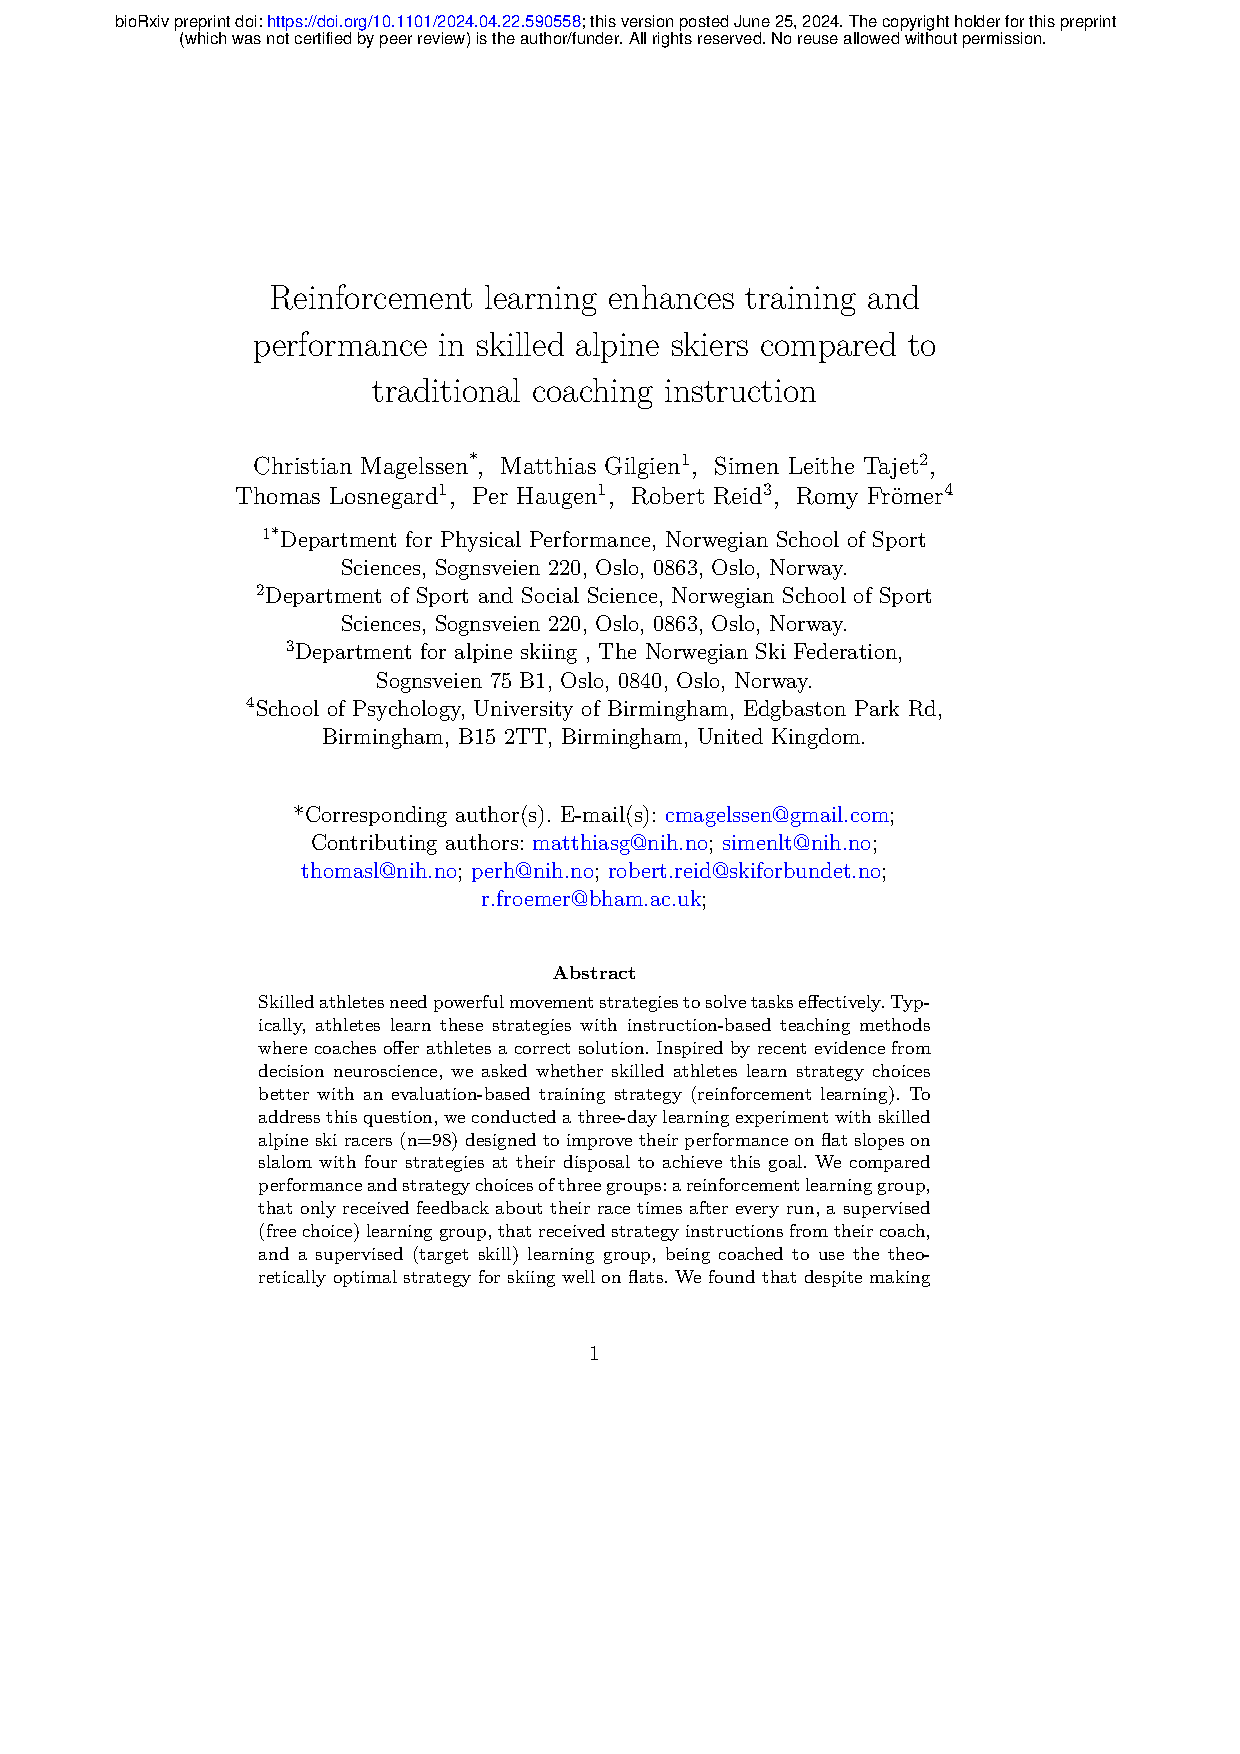
\includepdf[pages=-]{appendix/papers/paper_3.pdf}




\printbibliography

\end{document}
